\documentclass[11pt,a4paper]{article}
\usepackage[margin=2.2cm]{geometry}
\usepackage{amsmath,amssymb}
\usepackage{graphicx}
\usepackage{booktabs}
\usepackage{siunitx}
\usepackage{xcolor}
\usepackage{hyperref}
\usepackage{caption}
\usepackage[section]{placeins}
\graphicspath{{figs/}}
\newcommand{\HH}{H/H_0}

\title{Robustness of the SHiP muon shield to parameter tolerances}
\author{}
\date{\today}

\begin{document}
\maketitle

\begin{abstract}
How much do the muon hits on the SHiP sensitive plane change when the 50 free parameters of the
optimised muon shield (including the height of each magnet) deviate from their nominal values?
The muons come from a generative flow, each with its momentum and its production point in the
target. A neural surrogate of the per-muon hit probability (an ensemble of four DeepONets) gives
the gradient, the Hessian and candidate worst-case directions, and every conclusion is checked
with the full simulation on $10^9$ muons. The nominal design gives about $1240$ hits per $10^9$
muons. If every parameter may be off by up to $\varepsilon$, the worst design found within these
tolerances (searched on the surrogate, then simulated) multiplies the hits by $1.74\pm0.06$ at
$\varepsilon=1\%$, $3.9\pm0.1$ at $2\%$, $9.7\pm0.3$ at $3\%$, $121\pm3$ at $5\%$ and
$2840\pm80$ at $10\%$. A single parameter at its $\pm10\%$ limit gives at most $\times2.6\pm0.1$
(the entrance width of M2); the magnet heights matter least, at most $3\%$ each. Random
independent deviations are much milder: harmless at $\pm2\%$, mostly harmless at $\pm5\%$, with
a heavy tail at $\pm10\%$. Bounding the worst case takes sub-percent tolerances on a few
parameters, mostly of M2, M3 and M7: the allocation found for at most $\times2$ (simulated:
$\times1.56$) holds M2's entrance width, M3's inner yoke and field, and M7's field, length and
exit width to $\pm0.5\%$. Near the nominal design every harmful direction acts through muons of
$30$--$75$\,GeV, while the muons above $125$\,GeV respond the opposite way.
\end{abstract}

\tableofcontents

%==============================================================================
\section{Setup}
%==============================================================================

\paragraph{The shield.}
The design is the optimised configuration (\texttt{try\_opt}) of seven magnets M1--M7 (M0 is
fixed), with 50 free parameters (Table~\ref{tab:params}): lengths \texttt{Z\_len} and gaps
\texttt{Z\_gap}, the transverse sizes \texttt{dXIn}, \texttt{dXOut}, the inner gaps
\texttt{gapIn}, \texttt{gapOut}, the yoke widths \texttt{dXYokeIn/Out}, the height
\texttt{dYIn} of each magnet (its exit height \texttt{dYOut} moves with it; all in cm) and the
field $B$ of each magnet (the \texttt{NI} column, the target field in tesla). Fields are uniform
within each magnet block; the cavern is included.

\paragraph{Tolerances.}
Each parameter may vary by $\pm10\%$ of its nominal value:
\begin{equation}
  \phi_i = \phi_{0,i}\,(1 + 0.1\,u_i), \qquad u_i\in[-1,1].
\end{equation}
$u=0$ is the nominal design and $u_i=\pm1$ puts parameter $i$ alone at its limit. A step of
$\|u\|=1$ is ``one tolerance unit'': as large as one parameter at its limit, but spread over all
of them (RMS change $1.4\%$ per parameter). The corners of the box are at $\|u\|=\sqrt{50}=7.1$.
M6 and M7 have negative fields, so a negative change of their $B$ lowers $|B|$.

\paragraph{Muons and figure of merit.}
Muons are drawn from the generative flow of \texttt{generator\_muons} (the physical flux): the
momentum and charge, then the production point given them. They start where they are produced,
along the target ($z$ from $-2.14$ to $0$\,m before the shield, median $-1.68$\,m) and around the
beam axis (median radius $5$\,cm). The figure of merit $H$ is the number of muons crossing the
last sensitive plane per $10^9$ muons. At the nominal design, five simulator runs on the muons of
the analysis give $1194$--$1304$ (each $\pm35$; the transport is stochastic) and four runs on
independent muons $1220$--$1268$, a hit rate of $1.25\times10^{-6}$; the surrogate gives $1251$.
Every simulator number uses $10^9$ muons, the same ones for all designs of a table, with Poisson
errors (the transport is stochastic, so this holds even on shared muons).

\paragraph{Changes from the first analysis.}
A first analysis placed every muon on axis at $z=-1$\,m and left the heights fixed (43
parameters). Starting the muons at their production points raises the nominal hits by $54\%$
($810\to1251$ on the surrogate), at all momenta (Sec.~\ref{sec:momentum}); the heights hardly
matter. The conclusions are
unchanged; the main difference is that M2's entrance width now overtakes M7's field as the most
sensitive single parameter.

%==============================================================================
\section{The surrogate}
%==============================================================================

\paragraph{Model.}
The surrogate (LCSO) models the hit probability of each muon $x$ for a design $u$,
\begin{equation}
  p(\text{hit}\mid x,u) = \sigma\!\big(b(u)\cdot t(x) + c\big),
\end{equation}
a DeepONet with a branch network $b$ for the design and a trunk network $t$ for the muon
($p_x$, $p_y$, $p_z$, its production point $x$, $y$, $z$, and charge). The hits $H(u)$ are the
integral of $p$ over the muons, a smooth function of $u$ with exact derivatives. Four DeepONets
(two hidden layers of 128 units, 32 features) are trained with different seeds and their logits
averaged; the average is itself a DeepONet with concatenated features. A seed whose final
validation loss is more than $10\%$ above the median of its siblings would be replaced by a new
one; none was ($0.0226$--$0.0234$). The rule uses only the held-out training designs, not the
references. Errors on surrogate quantities are the standard error of the four members: the
surrogate's own seed-to-seed uncertainty.

\paragraph{Training data.}
The training data are simulated once, in six pools (Table~\ref{tab:pools}), and reused for every
epoch; nothing is re-simulated during training. Each pool is a set of designs, each simulated
with its own fresh muons from the flow:
\begin{itemize}
  \item \emph{Designs.} $u=\delta\,s\,r$, with $s$ a scrambled Sobol point in $[-1,1]^{50}$ and
        $r$ uniform in $(0,1)$, for a region of half-width $\delta$ ($\delta=1$: the $\pm10\%$
        box). The radial factor $r$ concentrates the designs towards the nominal one: of the
        25\,024 drawn this way in the box, 7723 have every parameter within $\pm3\%$. The
        first 16 designs of each pool are the nominal design itself. The \emph{wide} pool
        ($\delta=2$) puts half of its designs beyond the box, so that the box edges are inside
        the data.
  \item \emph{Adaptive.} A first ensemble, trained on the other five pools, was run through the
        analysis; its worst designs within $\pm1$--$10\%$ and those of its three tolerance
        allocations (Sec.~\ref{sec:tolerance}), each with four points on its line from the
        nominal design and 12 perturbations within its box, and the 64 random designs on which
        its members disagreed most, were simulated as a seventh pool (200 designs). This is where
        the conclusions rest and where the surrogate is least sure.
  \item \emph{Earlier pools.} The two largest pools of the first analysis are reused: their
        designs get the nominal heights and their muons stay on axis at $z=-1$\,m. The hit
        probability is set mainly by the momentum, so they still inform the model; the new pools
        teach it the production point and the heights.
  \item \emph{Muons.} Drawn from the flow at a raised \emph{momentum} temperature $T$ (only the
        momentum part of the flow is tempered; the production point keeps its distribution given
        the momentum), which broadens the momentum spectrum and raises the hit rate from
        $1.25\times10^{-6}$ (the physical flux) to $1.7\times10^{-4}$ ($T=1.5$) and
        $2.0\times10^{-3}$ ($T=2$). This does not bias the model, which learns
        $p(\text{hit}\mid x,u)$ per muon; the temperature only decides where in momentum the
        training data is dense.
  \item \emph{Rows.} Every hit and $0.4\%$ of the misses are kept, a case-control sample; the
        logit is fitted with the offset $\log 250$, so the model remains one of the full
        probability.
  \item \emph{Split.} The designs, not the rows, are split: 37\,143 for training and 4127 held
        out for early stopping. The validation references of Sec.~\ref{sec:validation} are
        separate simulations, never used for training.
\end{itemize}
In all, $7.1\times10^{10}$ simulated muons give $7.9\times10^7$ hits and $3.6\times10^8$ rows.
At the physical flux, as many hits would need $6\times10^{13}$ muons, i.e.\ about $130\,000$
designs of $5\times10^8$ muons; the same number of simulated muons would buy only $\sim140$
such designs.

\begin{table}[h]
\centering
\caption{Training pools. Designs are drawn in the region given, pulled towards the nominal
design except in the adaptive pool (see text); one design of each $T=2$ pool crashed the
simulator and is missing. The first-analysis pools have nominal heights and on-axis muons.}
\label{tab:pools}
\begin{tabular}{lrrrrr}
\toprule
pool & designs & muons per design & momentum $T$ & region & hits \\
\midrule
many designs   & 23\,999 & $10^6$ & 2   & $\pm10\%$ & $4.7\times10^7$ \\
wide           & 3999    & $10^6$ & 2   & $\pm20\%$ & $8.9\times10^6$ \\
main           & 1024    & $10^7$ & 1.5 & $\pm10\%$ & $1.8\times10^6$ \\
adaptive       & 200     & $10^7$ & 1.5 & selected  & $5.1\times10^5$ \\
\midrule
many designs, first analysis & 10\,000 & $10^6$ & 2   & $\pm10\%$ & $1.8\times10^7$ \\
main, first analysis         & 2048    & $10^7$ & 1.5 & $\pm10\%$ & $3.0\times10^6$ \\
\midrule
total          & 41\,270 & $7.1\times10^{10}$ & & & $7.9\times10^7$ \\
\bottomrule
\end{tabular}
\end{table}

\paragraph{Integration over the muons.}
A muon's momentum, azimuth and charge are independent in the flow: $(p_z,p_t)$ is the image of a
2-d standard normal latent. The surrogate's hits, gradient, Hessian and per-momentum splits are
therefore computed on a quadrature grid (latent $\times$ azimuth $\times$ charge,
App.~\ref{app:quadrature}) instead of by sampling muons, with one production point per grid node
drawn from the flow once, from a fixed seed. The grid reproduces a much finer one to
$4\times10^{-4}$ in $H$ and $2\times10^{-3}$ in the derivatives, where $10^9$ sampled muons leave
$1$--$2\%$ of noise. Only the simulator uses sampled muons.

\subsection{Validation against the simulator}
\label{sec:validation}

Reference designs were simulated on stored muons, on which the surrogate also predicts:
$6\times10^8$ muons of the physical flux (the nominal design four times, 16 designs in the half
box $|u_i|\le\tfrac12$, 16 in the box), and a high-momentum check sample of $4\times10^8$ muons
drawn like the $T=1.5$ pools ($\sim6\times10^4$ hits per design, so precise enough for
one-at-a-time effects: the same designs plus every parameter alone at $\pm10\%$).
Table~\ref{tab:val} and Fig.~\ref{fig:val} compare the surrogate with the simulator on them.

\begin{table}[t]
\centering
\caption{Surrogate vs.\ simulator on the reference designs: median $|\log(\text{pred}/\text{sim})|$
(signed for the nominal design), and the relative vector errors of the 50 one-at-a-time (OAT)
secants $\tfrac12[H(+e_i)-H(-e_i)]$ and curvatures $H(+e_i)+H(-e_i)-2H_0$ on the check sample.
``Noise'': what a perfect model would score, from the simulator's Poisson noise.}
\label{tab:val}
\begin{tabular}{lcc}
\toprule
 & noise & surrogate \\
\midrule
Nominal design                  & $1.8\%$  & $+0.2\%$ \\
Designs in the half box         & $2.2\%$  & $4.0\%$ \\
Designs in the box              & $1.8\%$  & $6.0\%$ \\
Check sample: nominal design    & $0.2\%$  & $-0.1\%$ \\
Check sample: designs in the box & $0.26\%$ & $1.8\%$ \\
OAT secants (cosine)            & $1.7\%$  & $2.6\%$ (0.9997) \\
OAT curvatures (cosine)         & $9.7\%$  & $12\%$ (0.993) \\
\bottomrule
\end{tabular}
\end{table}

\begin{figure}[t]
  \centering
  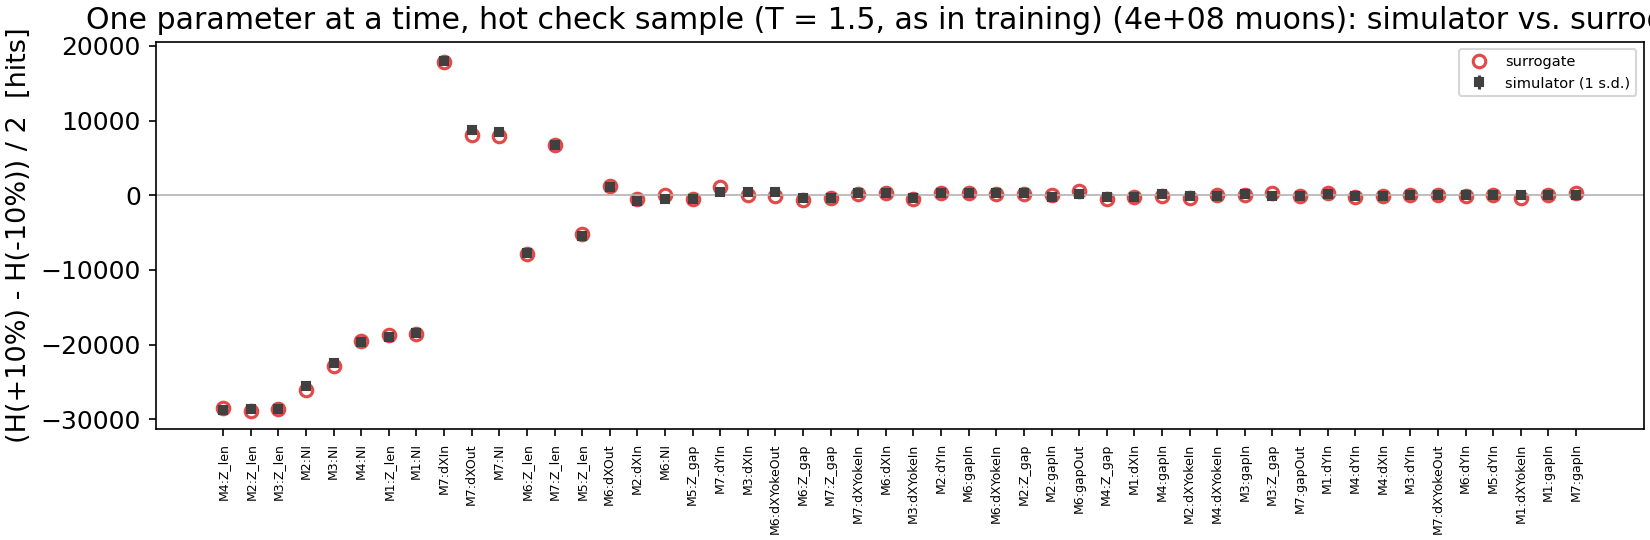
\includegraphics[width=\linewidth]{validation_oat.png}\\[1ex]
  \includegraphics[width=0.75\linewidth]{validation_calibration.png}
  \caption{Top: every parameter alone at $\pm10\%$, secant $\tfrac12[H(+10\%)-H(-10\%)]$ on the
  check sample: simulator (squares) and surrogate (circles). Bottom: predicted vs.\ simulated hits
  of the reference designs.}
  \label{fig:val}
\end{figure}

The one-at-a-time effects are reproduced to $2.6\%$, the designs in the half box to $4\%$ and in
the box to $6\%$, against $13\%$ in the first analysis: the wide and adaptive pools put data where
it was missing. The largest miss is the box design with the most hits, about $40\%$ low: far from
the nominal design the hits come mostly from muons of $30$--$75$\,GeV, which are rare in every
training sample. Within one tolerance unit, where the derivatives are read, the walks of
Sec.~\ref{sec:walks} agree with the simulator to $1$--$2\sigma$.

The derivatives are well determined: the four members' gradients at $u=0$ agree to
$\cos=0.96$--$0.99$ with the ensemble's. How the architecture and training were chosen is
summarised in App.~\ref{app:study}.

%==============================================================================
\section{Method}
%==============================================================================

From the surrogate we compute
\begin{itemize}
  \item the gradient $g=\nabla_u H$ and Hessian $\nabla^2_u H$ at $u=0$, and the exact
        one-at-a-time change $H(\pm e_i)/H_0-1$ of each parameter at its limit;
  \item the active subspace, the eigenvectors of $C=\mathbb{E}_x[\nabla_u p\,\nabla_u p^\top]$:
        the directions in which the hit probability of individual muons changes most;
  \item candidate worst directions, each of unit length:
    \texttt{ascent} ($v\propto g$),
    \texttt{worst} (maximiser of the quadratic model $g\cdot v+\tfrac12 v^\top\nabla^2H\,v$ on
    $\|v\|=1$),
    \texttt{hess1} (top Hessian eigenvector), \texttt{act1}, \texttt{act2} (top active
    directions), \texttt{corner} ($v\propto\operatorname{sign} g$: every parameter moved by the
    same amount) and \texttt{random};
  \item the worst corner of the box, by projected-gradient ascent (\texttt{pga});
  \item 4096 random designs in the box;
  \item the worst design for a given tolerance and a tolerance allocation
        (Sec.~\ref{sec:tolerance}).
\end{itemize}
Each direction is then walked, $u=t\,v$ for $t\in\{-1,-\tfrac12,\tfrac12,1\}$ (for \texttt{pga},
up to the box face), and simulated.

%==============================================================================
\section{Results}
%==============================================================================

\subsection{Single parameters}

33 of the 50 one-at-a-time effects are resolved beyond three times the members' scatter
(Fig.~\ref{fig:sensitivity}, Table~\ref{tab:oat}). The most sensitive parameter is the
\emph{entrance width of M2}: narrowed by $10\%$, it more than doubles the hits. Next come the
field of M7 (lowered by $10\%$: $\times1.9$), the length, exit width and yokes of M7, the inner
yoke, field and entrance width of M3, and the length of M6. Most responses are one-sided: one side
of the tolerance hardly matters, the other is harmful. A few (the lengths of M2 and M3, the field
of M3) are harmful on both sides, i.e.\ the nominal value sits near their minimum. Per magnet
(Fig.~\ref{fig:magnets}), M7 carries the largest share of the gradient ($71\%$ of its norm), then
M2 ($50\%$), M3 ($38\%$) and M6 ($23\%$). The \emph{heights} are the least sensitive parameters:
none changes the hits by more than $3\%$ at its limit (M2's: $+3.0\pm0.5\%$ at $+10\%$), and none
ranks above 23rd.

\paragraph{Simulated.} The eight largest were simulated at their worse limit
(Table~\ref{tab:concrete}): all eight rise significantly, five within $1$--$2\sigma$ of the
surrogate; the entrance width of M2 ($\times2.60\pm0.09$ vs.\ $2.30$), the exit width of M7
($1.70\pm0.06$ vs.\ $1.49$) and its inner yoke widened ($1.57\pm0.06$ vs.\ $1.35$) rise more than
predicted. Their scans were also simulated at $\pm5\%$ and $\pm10\%$ (Fig.~\ref{fig:scans}): 28
of the 32 points agree within $2\sigma$, and all 16 at $\pm5\%$. The misses are at $-10\%$, where
the surrogate is too smooth: M2's entrance width ($2.51$ simulated vs.\ $2.30$), M7's exit width
($1.64$ vs.\ $1.49$) and M7's inner yoke, which is harmful on both sides in the simulator
($1.19$ at $-10\%$ and $1.47$ at $+10\%$, vs.\ $1.06$ and $1.35$).

\begin{table}[t]
\centering
\caption{The most sensitive parameters (surrogate): first-order sensitivity $g_i/H_0$ per full
tolerance, and the exact change at $\pm10\%$ (errors: the members' standard error).}
\label{tab:oat}
\begin{tabular}{lrrrr}
\toprule
parameter & nominal & $g_i/H_0$ & $H/H_0-1$ at $+10\%$ & at $-10\%$ \\
\midrule
M2:\texttt{dXIn}       & 68.04 cm & $-0.507$ & $-0.01\pm0.06$ & $+1.30\pm0.07$ \\
M7:$B$                 & $-1.9$ T & $-0.457$ & $-0.24\pm0.02$ & $+0.92\pm0.06$ \\
M7:\texttt{Z\_len}     & 193.1 cm & $-0.385$ & $-0.22\pm0.01$ & $+0.69\pm0.03$ \\
M3:\texttt{dXYokeIn}   & 85.88 cm & $-0.324$ & $-0.08\pm0.03$ & $+0.53\pm0.03$ \\
M7:\texttt{dXOut}      & 67.81 cm & $-0.278$ & $-0.13\pm0.03$ & $+0.49\pm0.10$ \\
M3:$B$                 & 1.9 T    & $+0.153$ & $+0.37\pm0.05$ & $+0.04\pm0.03$ \\
M7:\texttt{dXYokeIn}   & 124.8 cm & $+0.319$ & $+0.34\pm0.02$ & $+0.06\pm0.04$ \\
M3:\texttt{dXIn}       & 64.81 cm & $+0.177$ & $+0.30\pm0.04$ & $-0.06\pm0.05$ \\
M6:\texttt{Z\_len}     & 168.0 cm & $-0.209$ & $-0.17\pm0.01$ & $+0.26\pm0.02$ \\
M2:\texttt{Z\_len}     & 224.9 cm & $+0.100$ & $+0.25\pm0.04$ & $+0.11\pm0.03$ \\
M2:$B$                 & 1.9 T    & $-0.102$ & $-0.03\pm0.02$ & $+0.23\pm0.03$ \\
M7:\texttt{dXYokeOut}  & 94.92 cm & $+0.206$ & $+0.22\pm0.01$ & $-0.08\pm0.02$ \\
M1:$B$                 & 1.9 T    & $-0.153$ & $-0.12\pm0.02$ & $+0.21\pm0.03$ \\
M3:\texttt{Z\_len}     & 225.0 cm & $+0.070$ & $+0.20\pm0.04$ & $+0.11\pm0.03$ \\
M4:\texttt{Z\_len}     & 224.0 cm & $-0.062$ & $-0.02\pm0.02$ & $+0.18\pm0.03$ \\
\bottomrule
\end{tabular}
\end{table}

\begin{figure}[p]
  \centering
  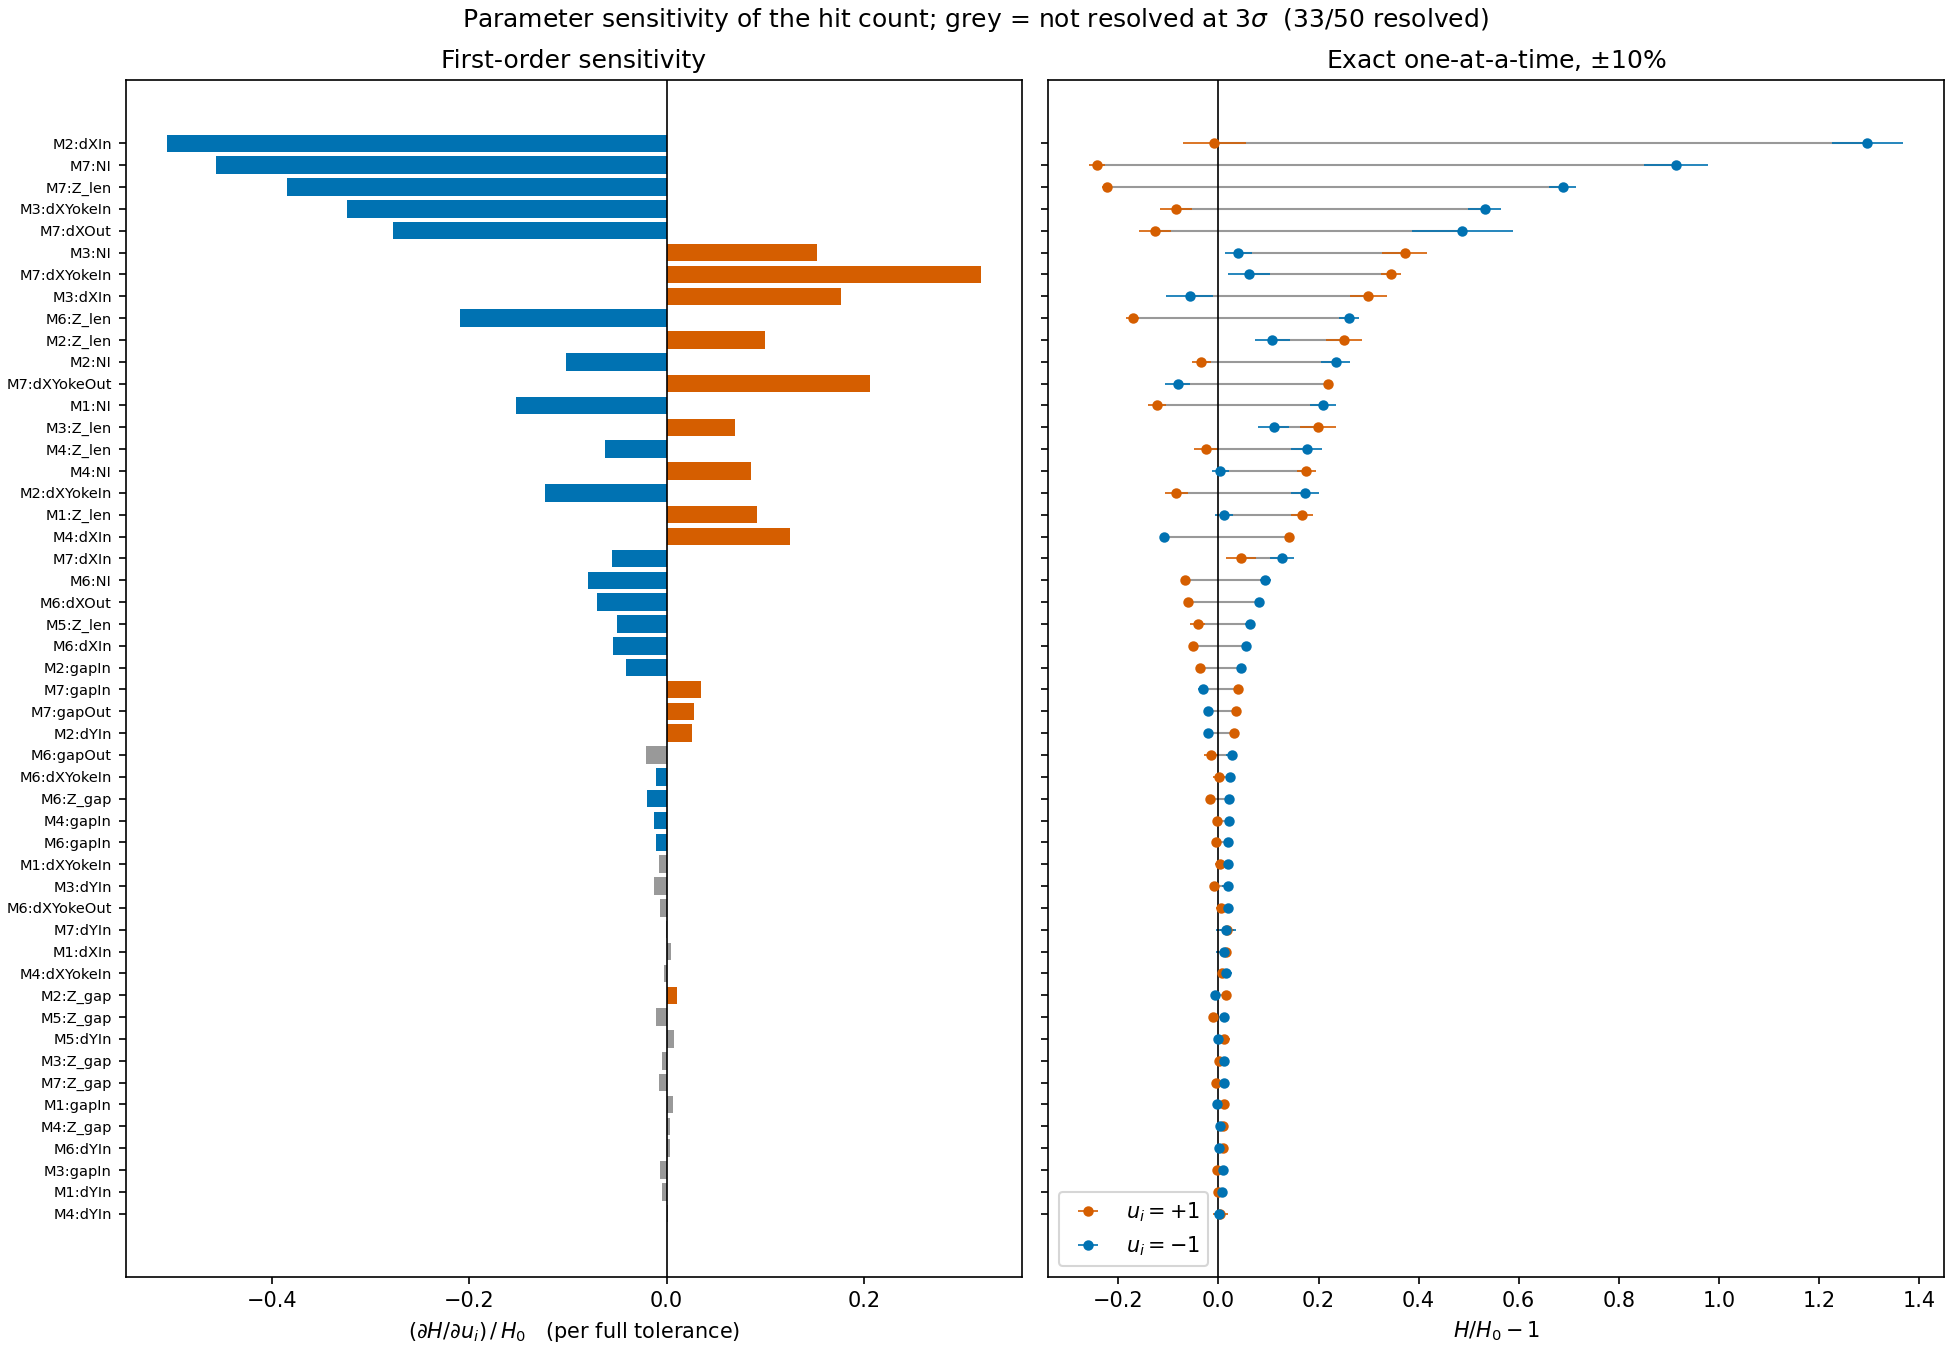
\includegraphics[width=\linewidth]{robustness_sensitivity.png}
  \caption{Sensitivity of each parameter. Left: gradient per full tolerance. Right: exact
  change with the parameter at $+10\%$ (orange) and $-10\%$ (blue).}
  \label{fig:sensitivity}
\end{figure}

\begin{figure}[t]
  \centering
  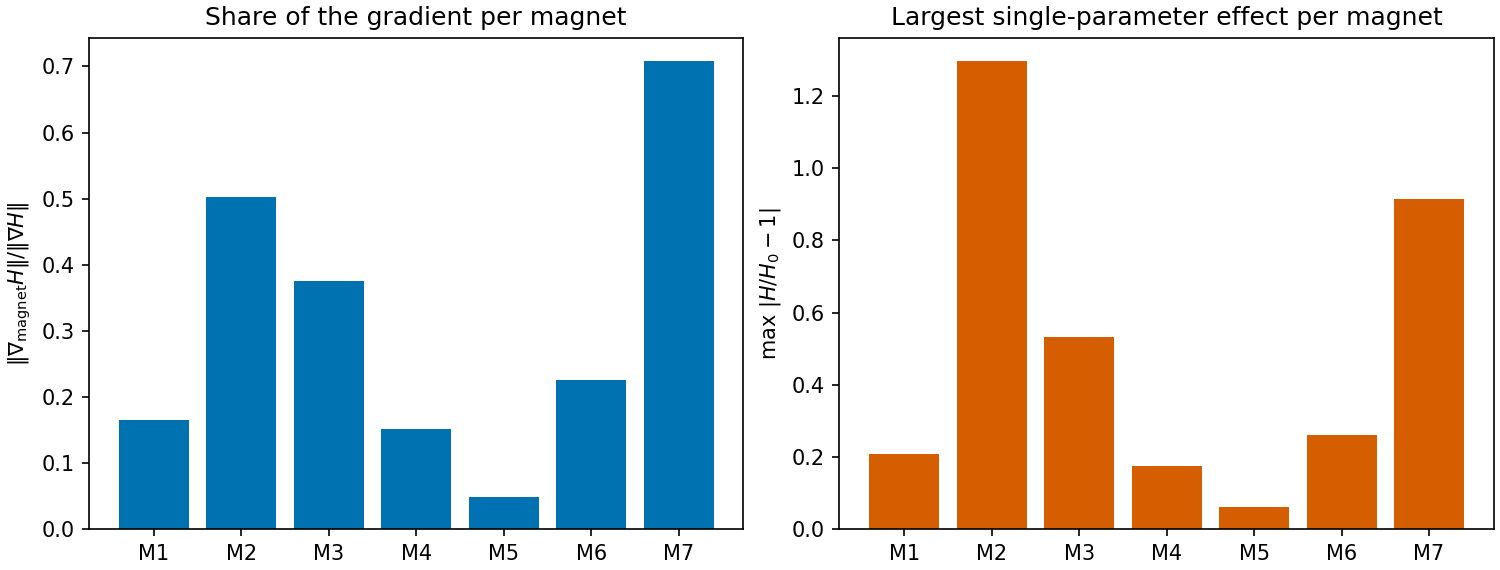
\includegraphics[width=0.8\linewidth]{robustness_magnets.png}
  \caption{Per magnet: share of the gradient norm and largest single-parameter effect.}
  \label{fig:magnets}
\end{figure}

\begin{figure}[t]
  \centering
  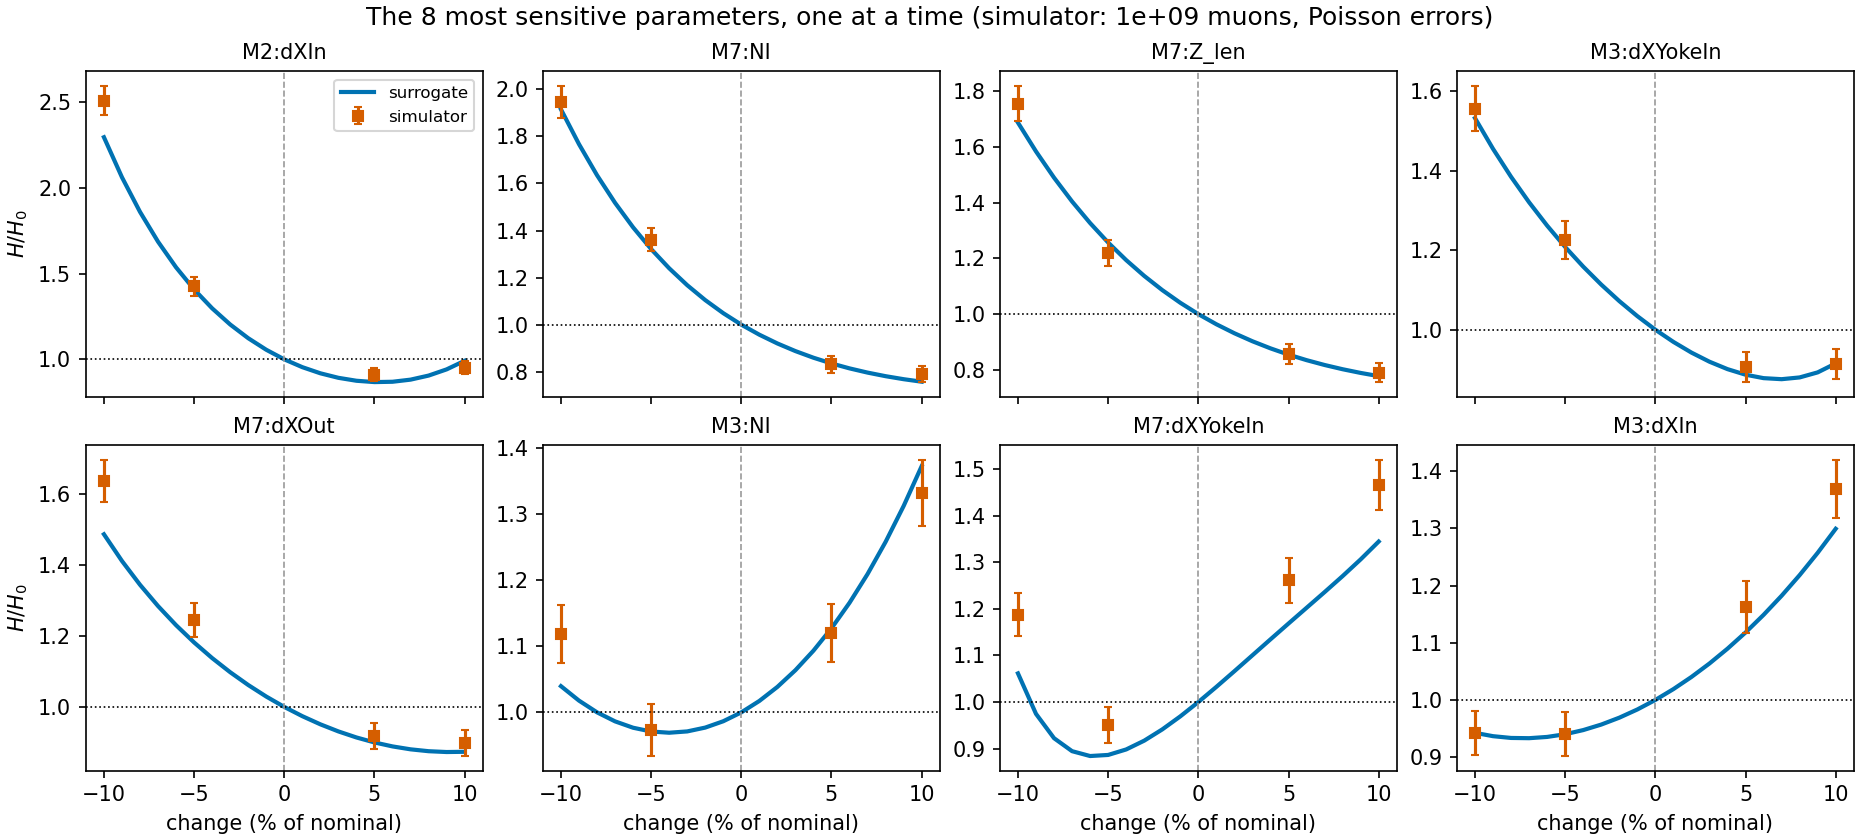
\includegraphics[width=\linewidth]{robustness_scans.png}
  \caption{One-at-a-time scans of the eight most sensitive parameters: surrogate (blue) and
  simulator at $\pm5\%$ and $\pm10\%$ (orange).}
  \label{fig:scans}
\end{figure}

\subsection{Curvature and active subspace}

One Hessian eigenvalue dominates (Fig.~\ref{fig:spectra}): $3.76\pm0.16\,H_0$ per unit$^2$, then
$0.90$, $0.59$ and $\lesssim0.17\,H_0$; 18 are negative, none below $-0.18\,H_0$. Along the
gradient the second-order term already exceeds the first-order one at one tolerance unit
($1.55\,H_0$ vs.\ $1.08\,H_0$): the response is strongly non-linear at that scale.

The active subspace is effectively one-dimensional ($98.4\%$ of $\mathbb{E}[\|\nabla_u p\|^2]$).
Its direction \texttt{act1} lengthens M1--M4 and raises their fields together, i.e.\ it changes
the upstream bending power (Table~\ref{tab:dirs}; the sign of an eigenvector is arbitrary). It is
almost orthogonal to the gradient ($\cos=0.17$): individual muons are deflected most along it,
but the changes largely cancel in the total.

\begin{figure}[t]
  \centering
  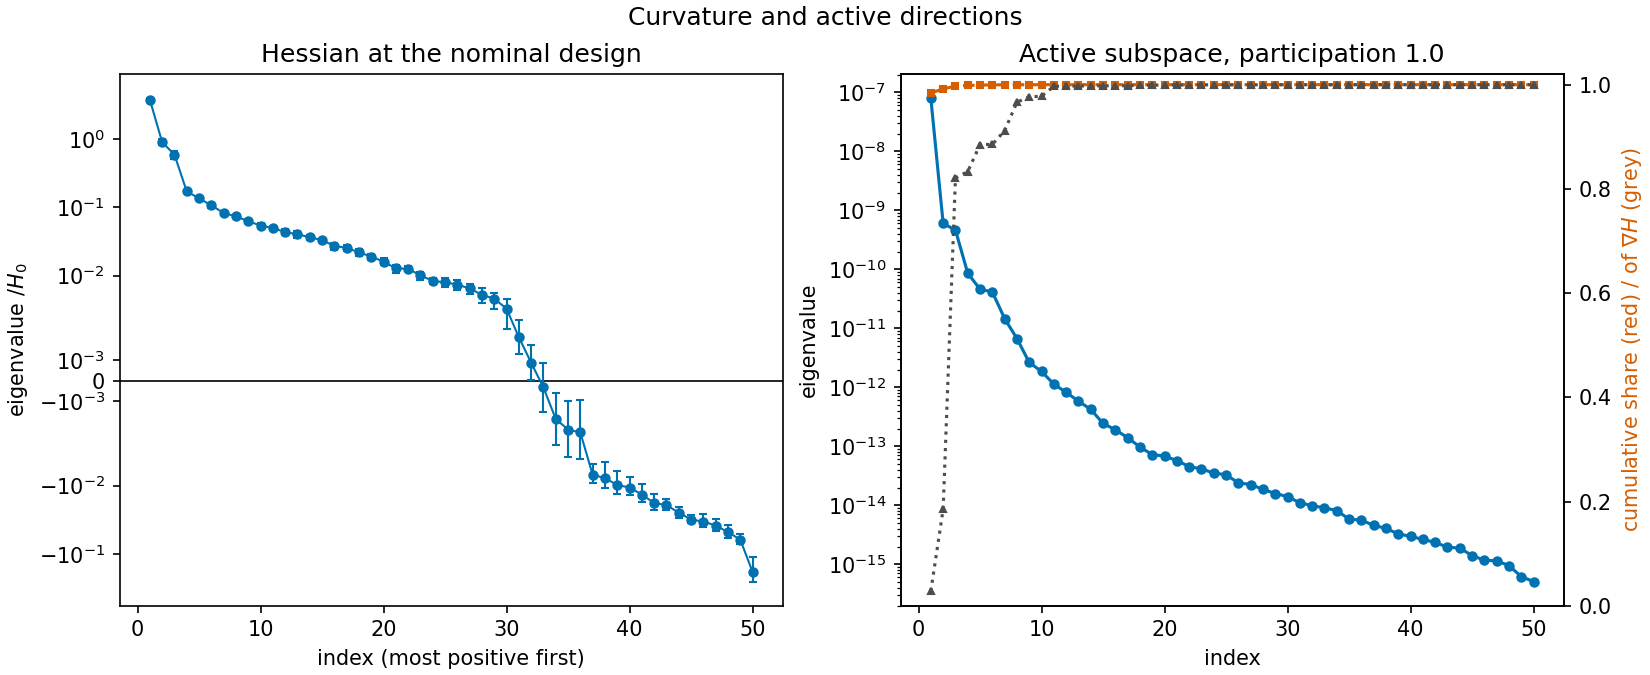
\includegraphics[width=0.9\linewidth]{robustness_spectra.png}
  \caption{Left: Hessian eigenvalues in units of $H_0$. Right: active-subspace eigenvalues
  (blue), their cumulative share (red) and the fraction of the gradient they contain (grey).}
  \label{fig:spectra}
\end{figure}

\subsection{Worst directions}
\label{sec:walks}

\begin{table}[t]
\centering
\caption{Hits one tolerance unit along each direction, surrogate and simulator (nominal: $1225$
simulated hits). ``max / RMS'': the largest and the RMS change over the 50 parameters.}
\label{tab:walks}
\small
\begin{tabular}{lcccrr}
\toprule
direction & max / RMS change & surrogate $\HH$ & simulator $\HH$ & sim.\ hits & at $t=-1$ (sim.) \\
\midrule
\texttt{hess1}  & 4.8\% / 1.4\% & $5.83\pm0.37$ & $5.61\pm0.17$ & 6871 & $1.22\pm0.05$ \\
\texttt{worst}  & 4.9\% / 1.4\% & $5.83\pm0.36$ & $5.57\pm0.17$ & 6818 & $1.05\pm0.04$ \\
\texttt{ascent} & 4.7\% / 1.4\% & $4.93\pm0.21$ & $5.01\pm0.16$ & 6140 & $0.76\pm0.03$ \\
\texttt{corner} & 1.4\% / 1.4\% & $2.52\pm0.08$ & $2.47\pm0.08$ & 3025 & $0.78\pm0.03$ \\
\texttt{act2}   & 6.3\% / 1.4\% & $2.22\pm0.09$ & $2.26\pm0.08$ & 2764 & $1.33\pm0.05$ \\
\texttt{act1}   & 3.9\% / 1.4\% & $1.84\pm0.09$ & $1.82\pm0.06$ & 2234 & $2.09\pm0.07$ \\
\texttt{random} & ---  / 1.4\% & $0.95\pm0.01$ & $0.94\pm0.04$ & 1152 & $1.25\pm0.05$ \\
\bottomrule
\end{tabular}
\end{table}

\paragraph{Small coordinated changes are far more harmful than a large single one.}
Moving every parameter by at most $4.9\%$ (RMS $1.4\%$) along \texttt{worst} multiplies the hits
by $5.6\pm0.2$ (Table~\ref{tab:walks}). The simplest such pattern, \texttt{corner}, moves
\emph{every} parameter by exactly $1.4\%$ with the sign of its gradient and gives $\times2.5$.
The worst single parameter needs a $10\%$ error for a similar effect. A random direction of the
same size changes little ($0.94\pm0.04$): the damage comes from the pattern of signs, not the size
of the step.

\paragraph{The surrogate gets both the directions and the sizes.}
Its two best directions (\texttt{worst} and \texttt{hess1}, $\cos=0.99$) are the two the
simulator ranks highest, then \texttt{ascent}. Within one tolerance unit it agrees with the
simulator to $1$--$2\sigma$ almost everywhere (Fig.~\ref{fig:calibration}); the exceptions are the
$t=-1$ ends of \texttt{ascent} ($1.02$ vs.\ $0.76\pm0.03$), \texttt{worst} ($1.27$ vs.\
$1.05\pm0.04$) and \texttt{random} ($1.12$ vs.\ $1.25\pm0.05$).

\paragraph{The quadratic model is not enough.}
Built from the gradient and Hessian, it underestimates every harmful direction ($3.9$ instead of
$5.6$ along \texttt{worst}, Fig.~\ref{fig:walks}): the hits grow roughly exponentially. The
derivatives give the directions; magnitudes come from the surrogate and the simulator.

\paragraph{The active subspace is a direction of curvature, not of slope.}
\texttt{act1} gives $\times1.82$ at $t=+1$ and $\times2.09$ at $t=-1$: lengthening or shortening
magnets 1--4 together, with their fields, is harmful either way, and the nominal design sits at
the balance point (Sec.~\ref{sec:momentum}). In the plane of \texttt{worst} and \texttt{act1}
(Fig.~\ref{fig:plane}) the nominal design lies in a shallow valley.

\begin{table}[t]
\centering
\caption{What each direction changes at one tolerance unit: its largest parameter changes,
relative and in physical units (cm, or T for $B$).}
\label{tab:dirs}
\small
\begin{tabular}{l p{0.55\linewidth} p{0.25\linewidth}}
\toprule
direction & largest changes & in words \\
\midrule
\texttt{worst}  & M2:\texttt{dXIn} $-4.9\%$ ($-3.3$), M7:$B$ $-3.6\%$ ($|B|$ $-0.07$ T),
                  M7:\texttt{Z\_len} $-3.4\%$ ($-6.5$), M3:\texttt{dXYokeIn} $-2.9\%$ ($-2.5$),
                  M3:$B$ $+2.6\%$ ($+0.05$ T), M2:\texttt{Z\_len} $+2.3\%$ ($+5.1$),
                  M7:\texttt{dXYokeIn} $+2.1\%$ ($+2.7$)
                & narrower M2 entrance, weaker and shorter M7, narrower M3 inner yoke \\
\midrule
\texttt{hess1}  & M2:\texttt{dXIn} $-4.8\%$ ($-3.3$), M7:$B$ $-3.3\%$ ($|B|$ $-0.06$ T),
                  M7:\texttt{Z\_len} $-3.2\%$ ($-6.1$), M3:$B$ $+2.9\%$ ($+0.06$ T),
                  M3:\texttt{dXYokeIn} $-2.8\%$ ($-2.4$), M2:\texttt{Z\_len} $+2.7\%$ ($+6.0$),
                  M3:\texttt{Z\_len} $+2.4\%$ ($+5.4$)
                & as \texttt{worst} \\
\midrule
\texttt{ascent} & M2:\texttt{dXIn} $-4.7\%$ ($-3.2$), M7:$B$ $-4.2\%$ ($|B|$ $-0.08$ T),
                  M7:\texttt{Z\_len} $-3.6\%$ ($-6.9$), M3:\texttt{dXYokeIn} $-3.0\%$ ($-2.6$),
                  M7:\texttt{dXYokeIn} $+3.0\%$ ($+3.7$), M7:\texttt{dXOut} $-2.6\%$ ($-1.8$),
                  M6:\texttt{Z\_len} $-1.9\%$ ($-3.3$)
                & the gradient: as \texttt{worst}, M7's yoke wider \\
\midrule
\texttt{corner} & all 50 parameters by exactly $\pm1.4\%$, each with the sign of its gradient
                & the simplest uniform pattern \\
\midrule
\texttt{act1}   & M2, M3, M4:\texttt{Z\_len} $+3.8$ to $+3.9\%$ ($+8.6$ to $+8.8$), M2:$B$ $+3.6\%$,
                  M3:$B$ $+3.2\%$, M4:$B$ $+2.8\%$ ($+0.05$ to $+0.07$ T), M1:\texttt{Z\_len}
                  $+2.6\%$ ($+4.0$)
                & magnets 1--4 longer and stronger: more bending upstream \\
\midrule
\texttt{act2}   & M7:\texttt{dXOut} $+6.3\%$ ($+4.3$), M7:\texttt{Z\_len} $-3.4\%$ ($-6.6$),
                  M7:\texttt{dXIn} $+3.2\%$ ($+1.2$), M2:\texttt{dXIn} $-3.1\%$ ($-2.1$),
                  M3:\texttt{dXYokeIn} $-2.5\%$ ($-2.1$), M6:\texttt{Z\_len} $-2.4\%$ ($-4.1$)
                & M7 wider and shorter, narrower M2 entrance \\
\bottomrule
\end{tabular}
\end{table}

\begin{figure}[p]
  \centering
  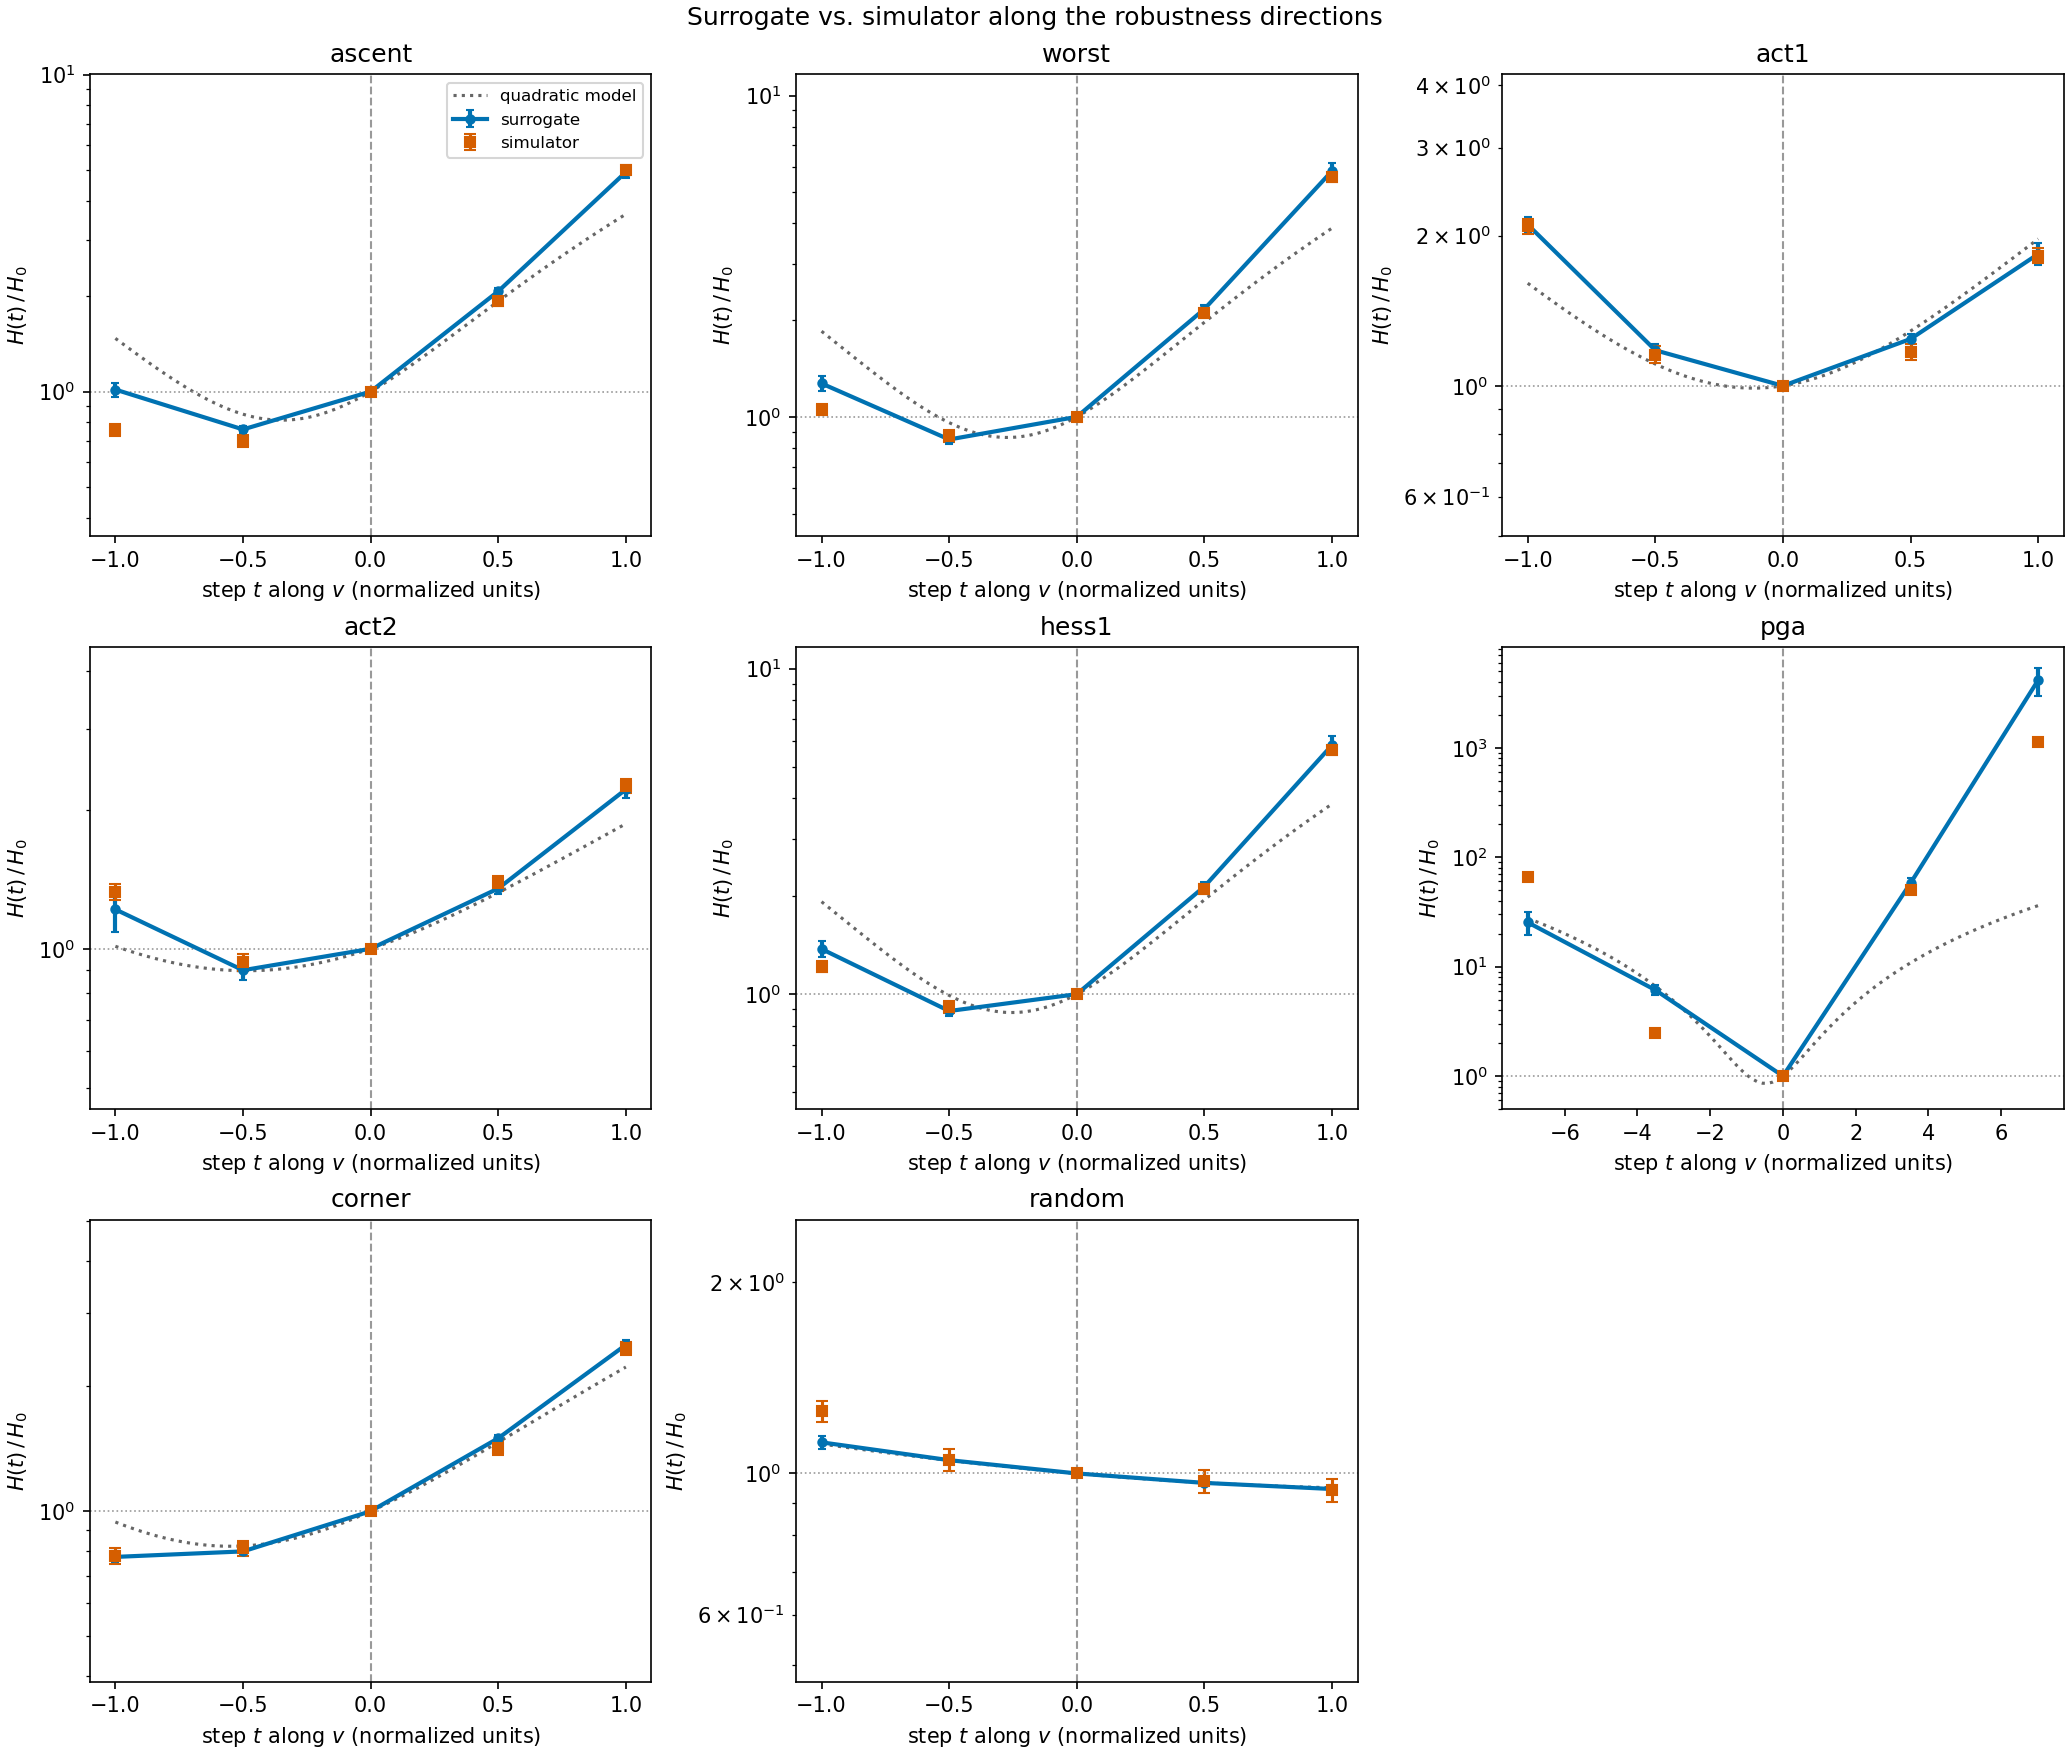
\includegraphics[width=\linewidth]{robustness_walks.png}
  \caption{Walks along each direction: surrogate (blue; error bars: the members), simulator
  (orange) and the quadratic model (dotted).}
  \label{fig:walks}
\end{figure}

\begin{figure}[t]
  \centering
  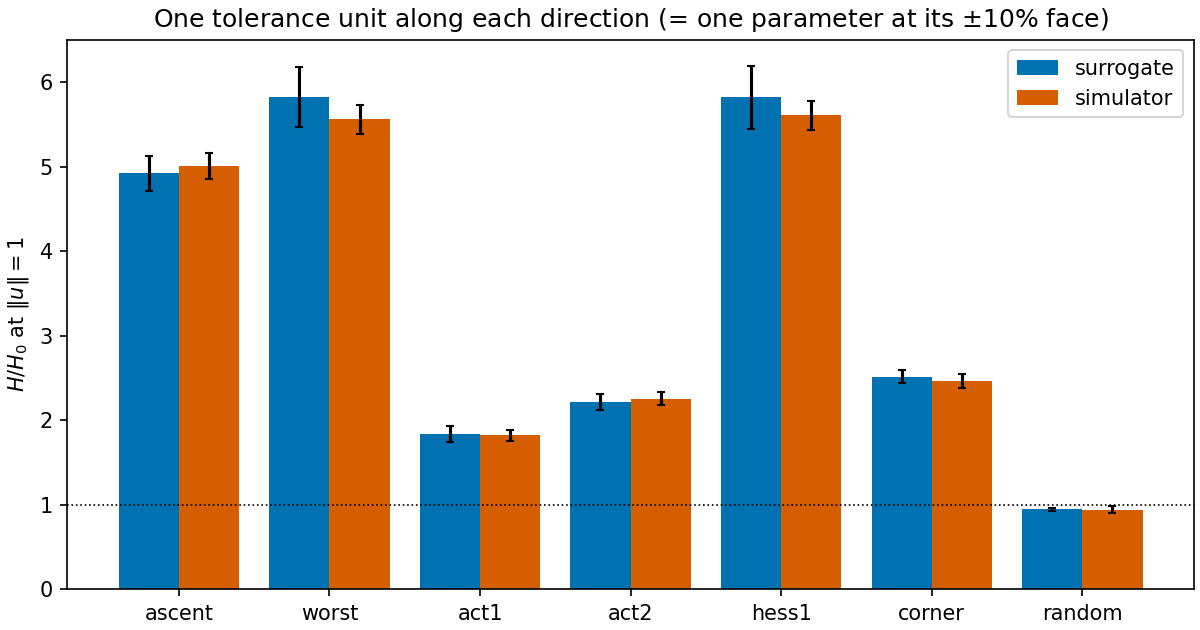
\includegraphics[width=0.48\linewidth]{robustness_summary.png}\hfill
  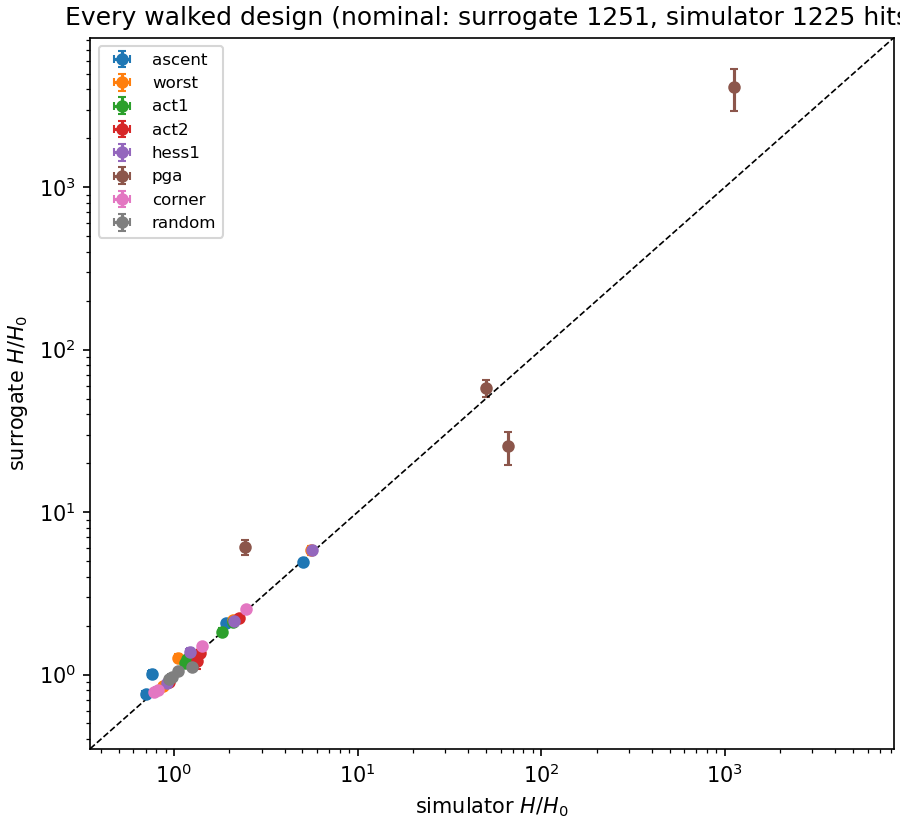
\includegraphics[width=0.42\linewidth]{robustness_calibration.png}
  \caption{Left: $\HH$ at one tolerance unit along each direction. Right: surrogate vs.\
  simulator for all 33 walked designs; the outliers are the box designs of Sec.~\ref{sec:box}.}
  \label{fig:calibration}
\end{figure}

\begin{figure}[t]
  \centering
  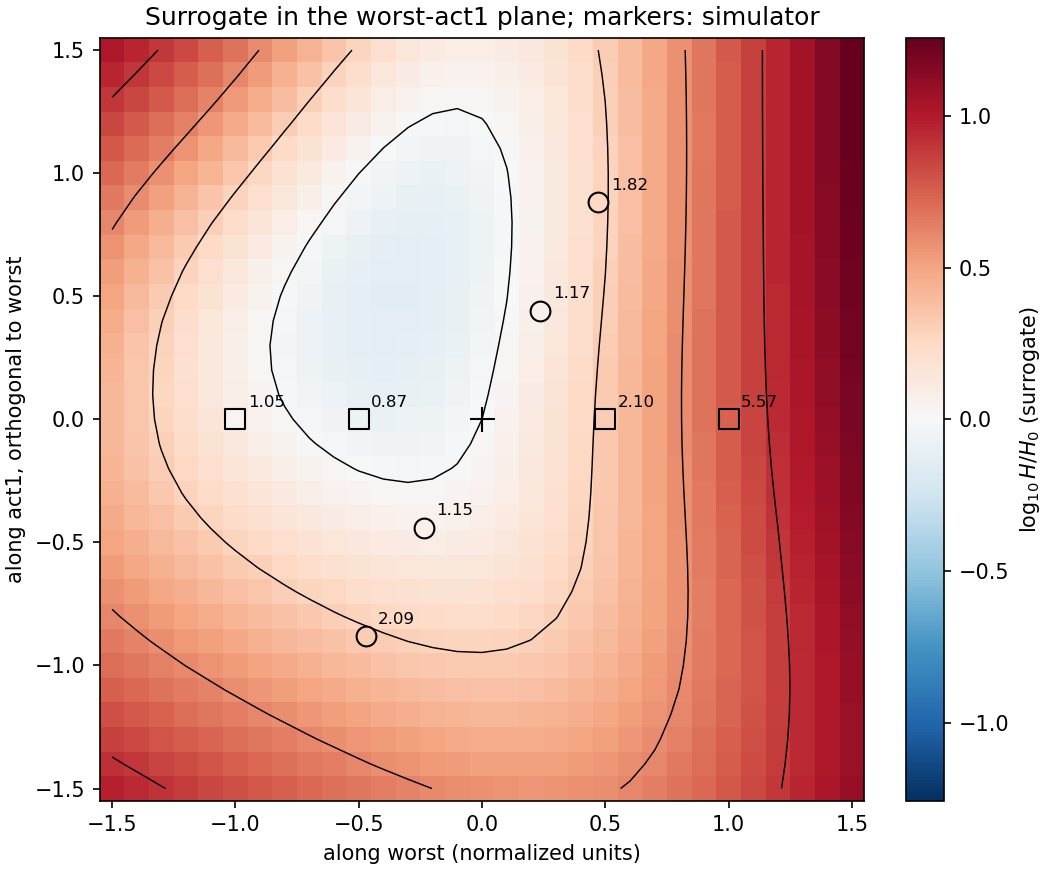
\includegraphics[width=0.6\linewidth]{robustness_plane.png}
  \caption{The surrogate in the plane of \texttt{worst} ($x$) and the part of \texttt{act1}
  orthogonal to it ($y$); markers: simulated designs with their $\HH$.}
  \label{fig:plane}
\end{figure}

\subsection{Concrete designs along the worst direction}
\label{sec:concrete}

Table~\ref{tab:concrete} lists concrete designs, all simulated. ``Worst, max $\varepsilon$'' is
the worst direction scaled so that no parameter moves by more than $\varepsilon$. It lies within
the $\pm\varepsilon$ tolerances, so it bounds their worst case from below; most of its
parameters stay well inside them, and the worst design within the tolerances is much worse
(Sec.~\ref{sec:tolerance}).

\begin{table}[t]
\centering
\caption{Concrete designs, simulated (nominal $1194\pm35$ hits) and predicted. At
$\varepsilon=10\%$ the worst direction changes M2:\texttt{dXIn} by $-6.8$ cm, $|B|$ of M7 from
$1.9$ to $1.76$ T, M7:\texttt{Z\_len} by $-13.4$ cm, M3:\texttt{dXYokeIn} by $-5.2$ cm,
M3:$B$ by $+0.10$ T, M2:\texttt{Z\_len} by $+10.6$ cm, M7:\texttt{dXYokeIn} by $+5.5$ cm,
M7:\texttt{dXOut} by $-2.9$ cm, M3:\texttt{dXIn} by $+2.7$ cm, M3:\texttt{Z\_len} by $+9.2$ cm,
and 40 more parameters by less than $3.4\%$.}
\label{tab:concrete}
\small
\begin{tabular}{llrcc}
\toprule
design & what changes & hits & sim.\ $\HH$ & surr.\ $\HH$ \\
\midrule
worst, max 1\%   & all 50, RMS 0.29\% & 1593  & $1.33\pm0.05$ & 1.30 \\
worst, max 2\%   & all 50, RMS 0.58\% & 2194  & $1.84\pm0.07$ & 1.84 \\
worst, max 3\%   & all 50, RMS 0.87\% & 3133  & $2.62\pm0.09$ & 2.73 \\
worst, max 5\%   & all 50, RMS 1.45\% & 7167  & $6.00\pm0.19$ & 6.19 \\
worst, max 10\%  & all 50, RMS 2.9\%  & 60879 & $51.0\pm1.5$  & 47.3 \\
opposite, max 5\% & all 50, signs reversed & 1300 & $1.09\pm0.04$ & 1.32 \\
opposite, max 10\% & all 50, signs reversed & 3545 & $2.97\pm0.10$ & 6.25 \\
\midrule
worst, top 1 only  & M2:\texttt{dXIn} $-10\%$ ($-6.8$ cm) & 3122 & $2.62\pm0.09$ & 2.30 \\
worst, top 3 only  & + M7:$B$ $-7.5\%$, M7:\texttt{Z\_len} $-6.9\%$ & 7010 & $5.87\pm0.18$ & 5.46 \\
worst, top 5 only  & + M3:\texttt{dXYokeIn} $-6\%$, M3:$B$ $+5.3\%$ & 14447 & $12.1\pm0.4$ & 10.3 \\
worst, top 10 only & the ten largest changes & 35362 & $29.6\pm0.9$ & 26.6 \\
\midrule
single & M2:\texttt{dXIn} $-10\%$ ($-6.8$ cm)   & 3109 & $2.60\pm0.09$ & 2.30 \\
single & M7:$B$ $-10\%$ ($|B|$ $1.9\to1.71$ T) & 2465 & $2.06\pm0.07$ & 1.92 \\
single & M7:\texttt{Z\_len} $-10\%$ ($-19.3$ cm) & 2131 & $1.79\pm0.07$ & 1.69 \\
single & M7:\texttt{dXOut} $-10\%$ ($-6.8$ cm)  & 2025 & $1.70\pm0.06$ & 1.49 \\
single & M7:\texttt{dXYokeIn} $+10\%$ ($+12.5$ cm) & 1878 & $1.57\pm0.06$ & 1.35 \\
single & M3:\texttt{dXYokeIn} $-10\%$ ($-8.6$ cm) & 1876 & $1.57\pm0.06$ & 1.53 \\
single & M3:$B$ $+10\%$ ($1.9\to2.09$ T) & 1686 & $1.41\pm0.05$ & 1.37 \\
single & M3:\texttt{dXIn} $+10\%$ ($+6.5$ cm) & 1666 & $1.40\pm0.05$ & 1.30 \\
\bottomrule
\end{tabular}
\end{table}

\paragraph{Exponential growth along the direction.}
Along the worst direction (Fig.~\ref{fig:scaled}) the hits grow by $\times1.33$ at a maximum
change of $1\%$, $\times1.8$ at $2\%$, $\times2.6$ at $3\%$, $\times6.0$ at $5\%$ and $\times51$ at
$10\%$: a factor $e$ per $\sim2.5\%$ of tolerance. The surrogate follows to within $5\%$ up to
$5\%$ and is $7\%$ low at $10\%$. The opposite direction is harmless at $5\%$ ($\times1.09$) but
not at $10\%$ ($\times3.0$, where the surrogate predicts $\times6.2$), through other muons
(Sec.~\ref{sec:momentum}).

\paragraph{The rise is collective.}
The largest component alone (M2:\texttt{dXIn} $-10\%$) gives $\times2.6$; the top three (adding a
weaker and shorter M7) $\times5.9$; the top five $\times12$; the top ten $\times30$; all 50
$\times51$ (Fig.~\ref{fig:attribution}). Each parameter contributes a moderate factor, and the
factors multiply.

\begin{figure}[t]
  \centering
  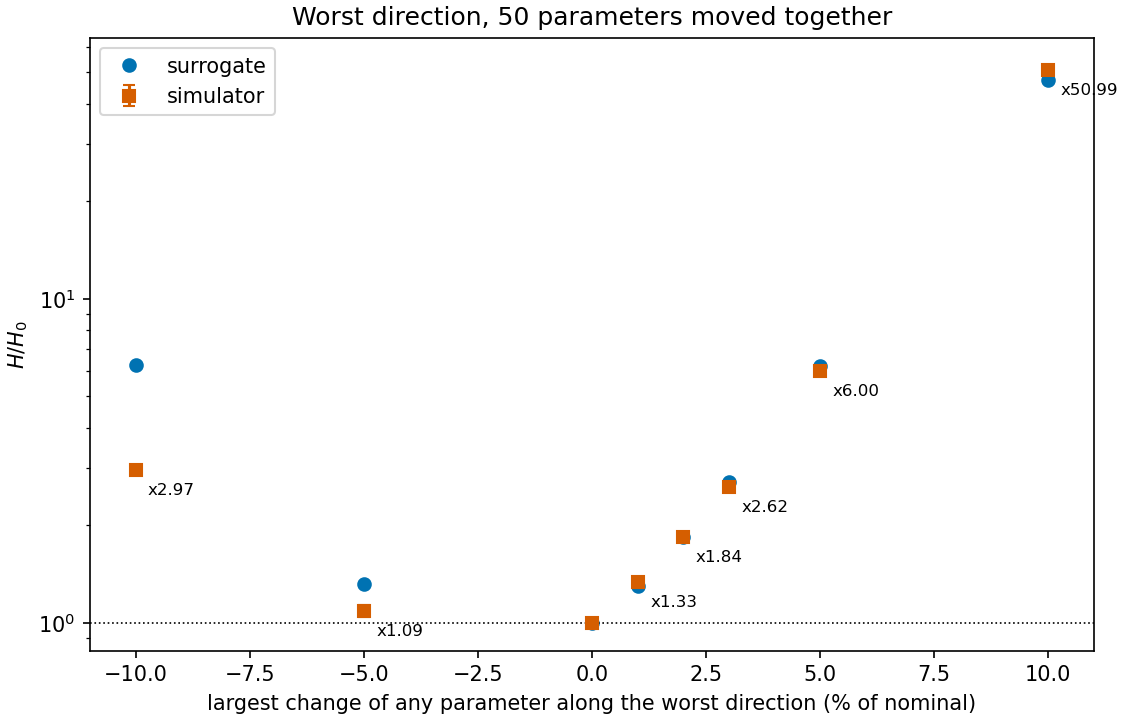
\includegraphics[width=0.7\linewidth]{worst_direction_scaled.png}
  \caption{Hits along the worst direction against the largest change of any parameter:
  simulator and surrogate.}
  \label{fig:scaled}
\end{figure}

\begin{figure}[t]
  \centering
  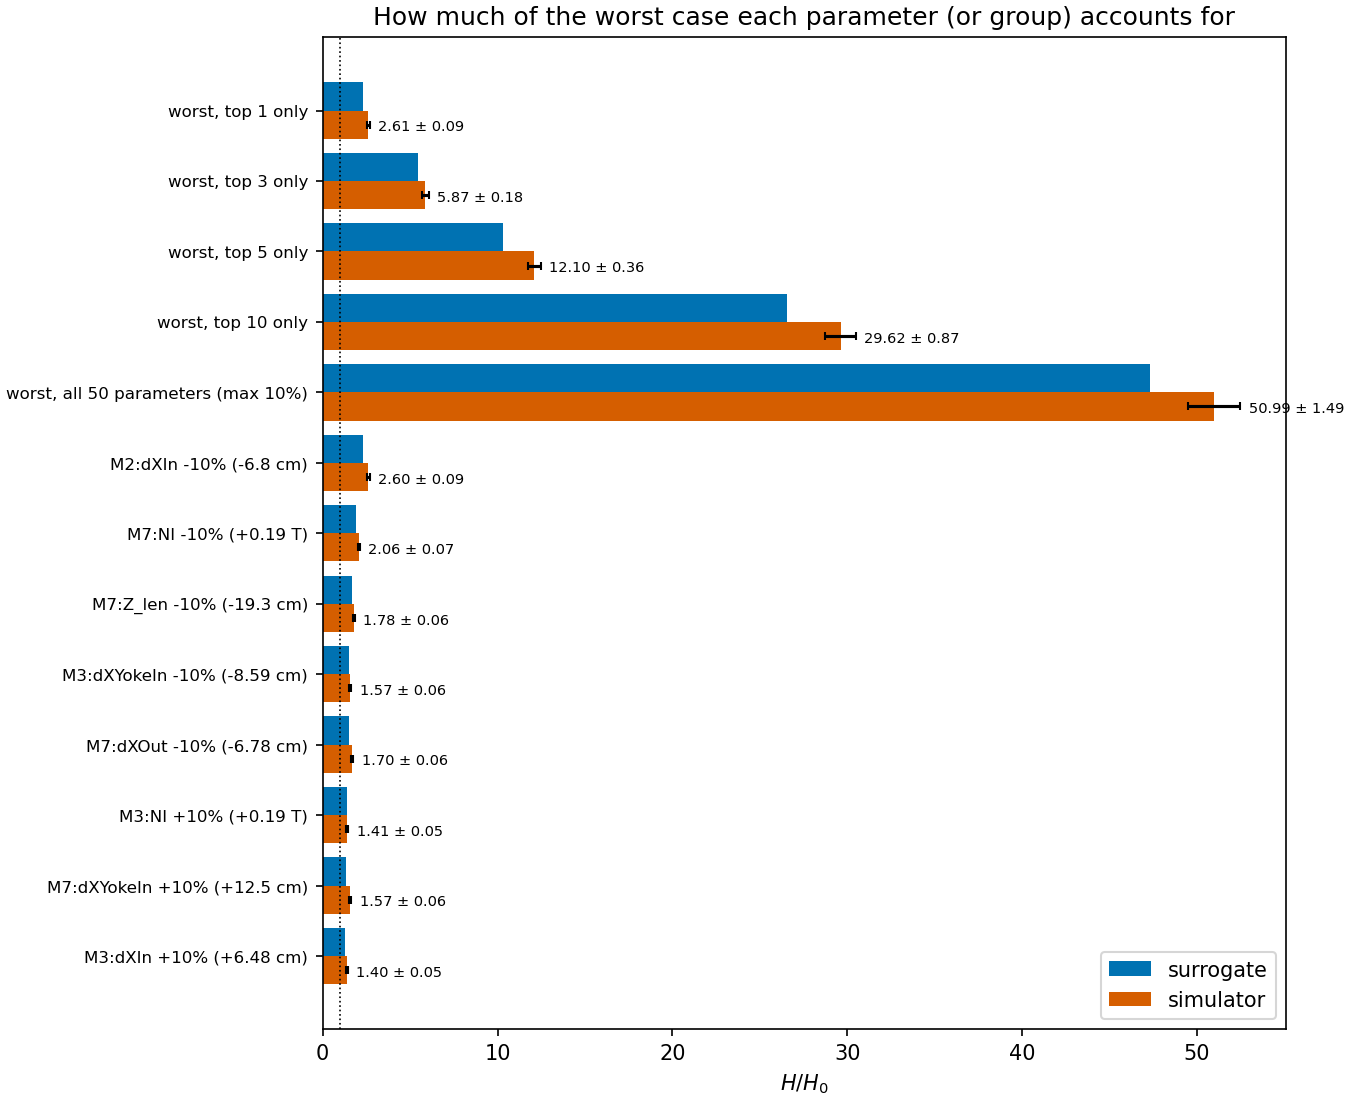
\includegraphics[width=0.8\linewidth]{worst_parameters.png}
  \caption{The worst direction at a maximum change of $10\%$, truncated to its largest 1, 3, 5,
  10 changes, and single parameters at their worse limit.}
  \label{fig:attribution}
\end{figure}

\FloatBarrier
\subsection{The worst case for a given tolerance}
\label{sec:tolerance}
\label{sec:box}

\paragraph{Method.} If every parameter may be off by up to $\varepsilon$, the designs allowed
form the box $|u_i|\le\varepsilon/10\%$. Its worst design is found on the surrogate, by
projected-gradient ascent of $\log H$ over the box from 16 starting points (the sign of the
gradient, the scaled worst direction and random corners; 300 Adam steps each, all batched,
seconds per box), and then simulated on $10^9$ muons. The simulated values are real designs
within the tolerances, so the true worst case is at least as bad; the search is as good as the
surrogate, which is accurate there up to $\pm3\%$ and overestimates beyond. The worst direction
of Sec.~\ref{sec:walks} maximises the hits on a sphere ($\|u\|=1$); on a box the maximum is at a
corner, every parameter at a limit with the harmful sign, so scaling the direction down
underestimates it.

\begin{table}[!htb]
\centering
\caption{The worst design within $\pm\varepsilon$ on every parameter: found on the surrogate,
simulated ($10^9$ muons; nominal $1304\pm36$). Last column: the worst direction scaled to the
same $\varepsilon$ (Table~\ref{tab:concrete}).}
\label{tab:tolerance}
\begin{tabular}{lrrccc}
\toprule
$\varepsilon$ & at a limit & sim.\ hits & sim.\ $\HH$ & surr.\ $\HH$ & scaled direction (sim.) \\
\midrule
$1\%$  & 50 & 2269        & $1.74\pm0.06$ & $1.88\pm0.05$ & $1.33\pm0.05$ \\
$2\%$  & 50 & 5032        & $3.86\pm0.12$ & $4.38\pm0.28$ & $1.84\pm0.07$ \\
$3\%$  & 49 & 12\,595     & $9.7\pm0.3$   & $10.8\pm0.7$  & $2.62\pm0.09$ \\
$5\%$  & 44 & 158\,129    & $121\pm3$     & $214\pm20$    & $6.00\pm0.19$ \\
$10\%$ & 46 & 3\,701\,210 & $2840\pm80$   & $(1.9\pm1.7)\times10^4$ & $51.0\pm1.5$ \\
\bottomrule
\end{tabular}
\end{table}

\begin{figure}[!htb]
  \centering
  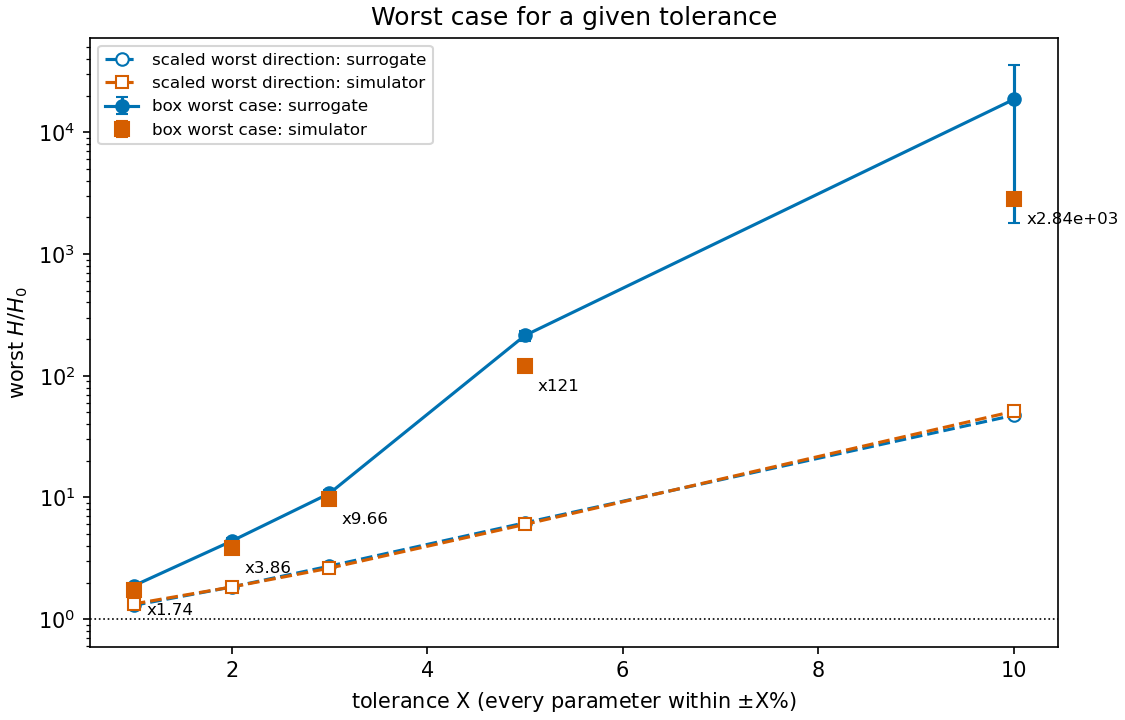
\includegraphics[width=0.75\linewidth]{tolerance_boxes.png}
  \caption{Worst case for a given tolerance: the worst design within $\pm\varepsilon$ (filled;
  surrogate and simulator) and the worst direction scaled to $\varepsilon$ (open).}
  \label{fig:tolerance}
\end{figure}

\paragraph{Results} (Table~\ref{tab:tolerance}, Fig.~\ref{fig:tolerance}). Already at $\pm1\%$
the worst design gives $\times1.7$, at $\pm2\%$ $\times3.9$ and at $\pm3\%$ $\times9.7$, $1.3$ to
four times the scaled direction. Up to $\pm3\%$ these designs act through the known mechanism:
the largest contributions are those of the worst direction (M2's entrance narrower, M7 weaker and
shorter, M3's inner yoke narrower and its field higher), but every parameter is at its limit
($\cos\approx0.6$ with the worst direction), and the surrogate predicts them to $8$--$13\%$, on the
high side. At $\pm5\%$ and $\pm10\%$ the search finds another mechanism, M7's yokes and exit
narrower with M2's entrance and M3's inner yoke wider ($\cos=-0.18$ and $-0.20$ with the worst
direction), which the local derivatives do not show; the simulated scans point the same way (M7's
inner yoke harmful on both sides, Fig.~\ref{fig:scans}). There the surrogate overestimates, by
$\times1.8$ at $\pm5\%$ and $\times7$ at $\pm10\%$ (in the first analysis $\times30$), but the
designs it finds are real: $\times121$ at $\pm5\%$ and $\times2840$ at $\pm10\%$. The cruder box
search of the walks (\texttt{pga}, 4 starts, 200 steps) ends at a corner with
$\times1125\pm32$, $90\%$ of it from muons of $40$--$60$\,GeV; halfway to it (every parameter at
$5\%$) the simulator gives $\times50\pm1.5$, and its opposite corner $\times66\pm2$ (surrogate:
$\times25$). Which muons make the hits of the $\pm5\%$ and $\pm10\%$ worst designs was not
measured.

\subsection{Tolerance allocation}
\label{sec:allocation}

\paragraph{Method.} Which tolerances keep the worst case below a target? Greedily: start with
every parameter at $\pm10\%$; find the box's worst design $u^*$ as above; tighten the two
parameters that contribute most to it (the largest first-order shares of $\log H$,
$u^*_i\,\partial\log H/\partial u_i$) by a factor $0.8$, down to a floor of $\pm0.5\%$; repeat
until the worst case is below the target. The first box that meets each target is its
allocation, and its worst design is simulated. This is a heuristic, not an optimum: other
allocations may loosen some parameters for the same target.

\begin{table}[!htb]
\centering
\caption{Tolerance allocations (greedy, surrogate) for a worst case of at most $3$, $2$ and $1.5$
times the nominal hits: the sixteen tightest parameters ($\pm\%$), and a summary of all 50. The
worst design of each allocation is simulated in the last row.}
\label{tab:allocation}
\small
\begin{tabular}{lrccc}
\toprule
parameter & nominal & $\le3H_0$ & $\le2H_0$ & $\le1.5H_0$ \\
\midrule
M2:\texttt{dXIn}         & 68.04 cm & 0.50 & 0.50 & 0.50 \\
M7:$B$                   & 1.9 T    & 0.55 & 0.50 & 0.50 \\
M7:\texttt{Z\_len}       & 193.1 cm & 0.55 & 0.50 & 0.50 \\
M3:\texttt{dXYokeIn}     & 85.88 cm & 0.69 & 0.50 & 0.50 \\
M7:\texttt{dXOut}        & 67.81 cm & 0.86 & 0.50 & 0.50 \\
M3:$B$                   & 1.9 T    & 0.86 & 0.50 & 0.50 \\
M3:\texttt{dXIn}         & 64.81 cm & 0.86 & 0.55 & 0.50 \\
M2:\texttt{Z\_len}       & 224.9 cm & 0.86 & 0.55 & 0.50 \\
M7:\texttt{dXYokeIn}     & 124.8 cm & 1.07 & 0.55 & 0.50 \\
M3:\texttt{Z\_len}       & 225.0 cm & 1.07 & 0.69 & 0.50 \\
M4:$B$                   & 1.9 T    & 1.07 & 0.69 & 0.50 \\
M6:\texttt{Z\_len}       & 168.0 cm & 1.07 & 0.69 & 0.50 \\
M1:\texttt{Z\_len}       & 151.5 cm & 1.34 & 0.86 & 0.50 \\
M7:\texttt{dXYokeOut}    & 94.92 cm & 1.68 & 0.86 & 0.50 \\
M4:\texttt{dXIn}         & 39.02 cm & 1.68 & 1.07 & 0.50 \\
M2:\texttt{dXYokeIn}     & 70.62 cm & 2.62 & 1.34 & 0.50 \\
\midrule
parameters below $\pm1\%$ / $\pm2\%$ / $\pm5\%$ & & 8 / 15 / 26 & 14 / 19 / 34 & 21 / 26 / 45 \\
median tolerance & & $4.1\%$ & $3.3\%$ & $1.7\%$ \\
heights (\texttt{dYIn}) & & $5.1$--$8\%$ & $4.1$--$8\%$ & $2.1$--$5.1\%$ \\
\midrule
worst design: surrogate & & $2.98\pm0.32$ & $1.99\pm0.09$ & $1.50\pm0.04$ \\
worst design: simulator & & $2.20\pm0.07$ & $1.56\pm0.06$ & $1.31\pm0.05$ \\
\bottomrule
\end{tabular}
\end{table}

\begin{figure}[!htbp]
  \centering
  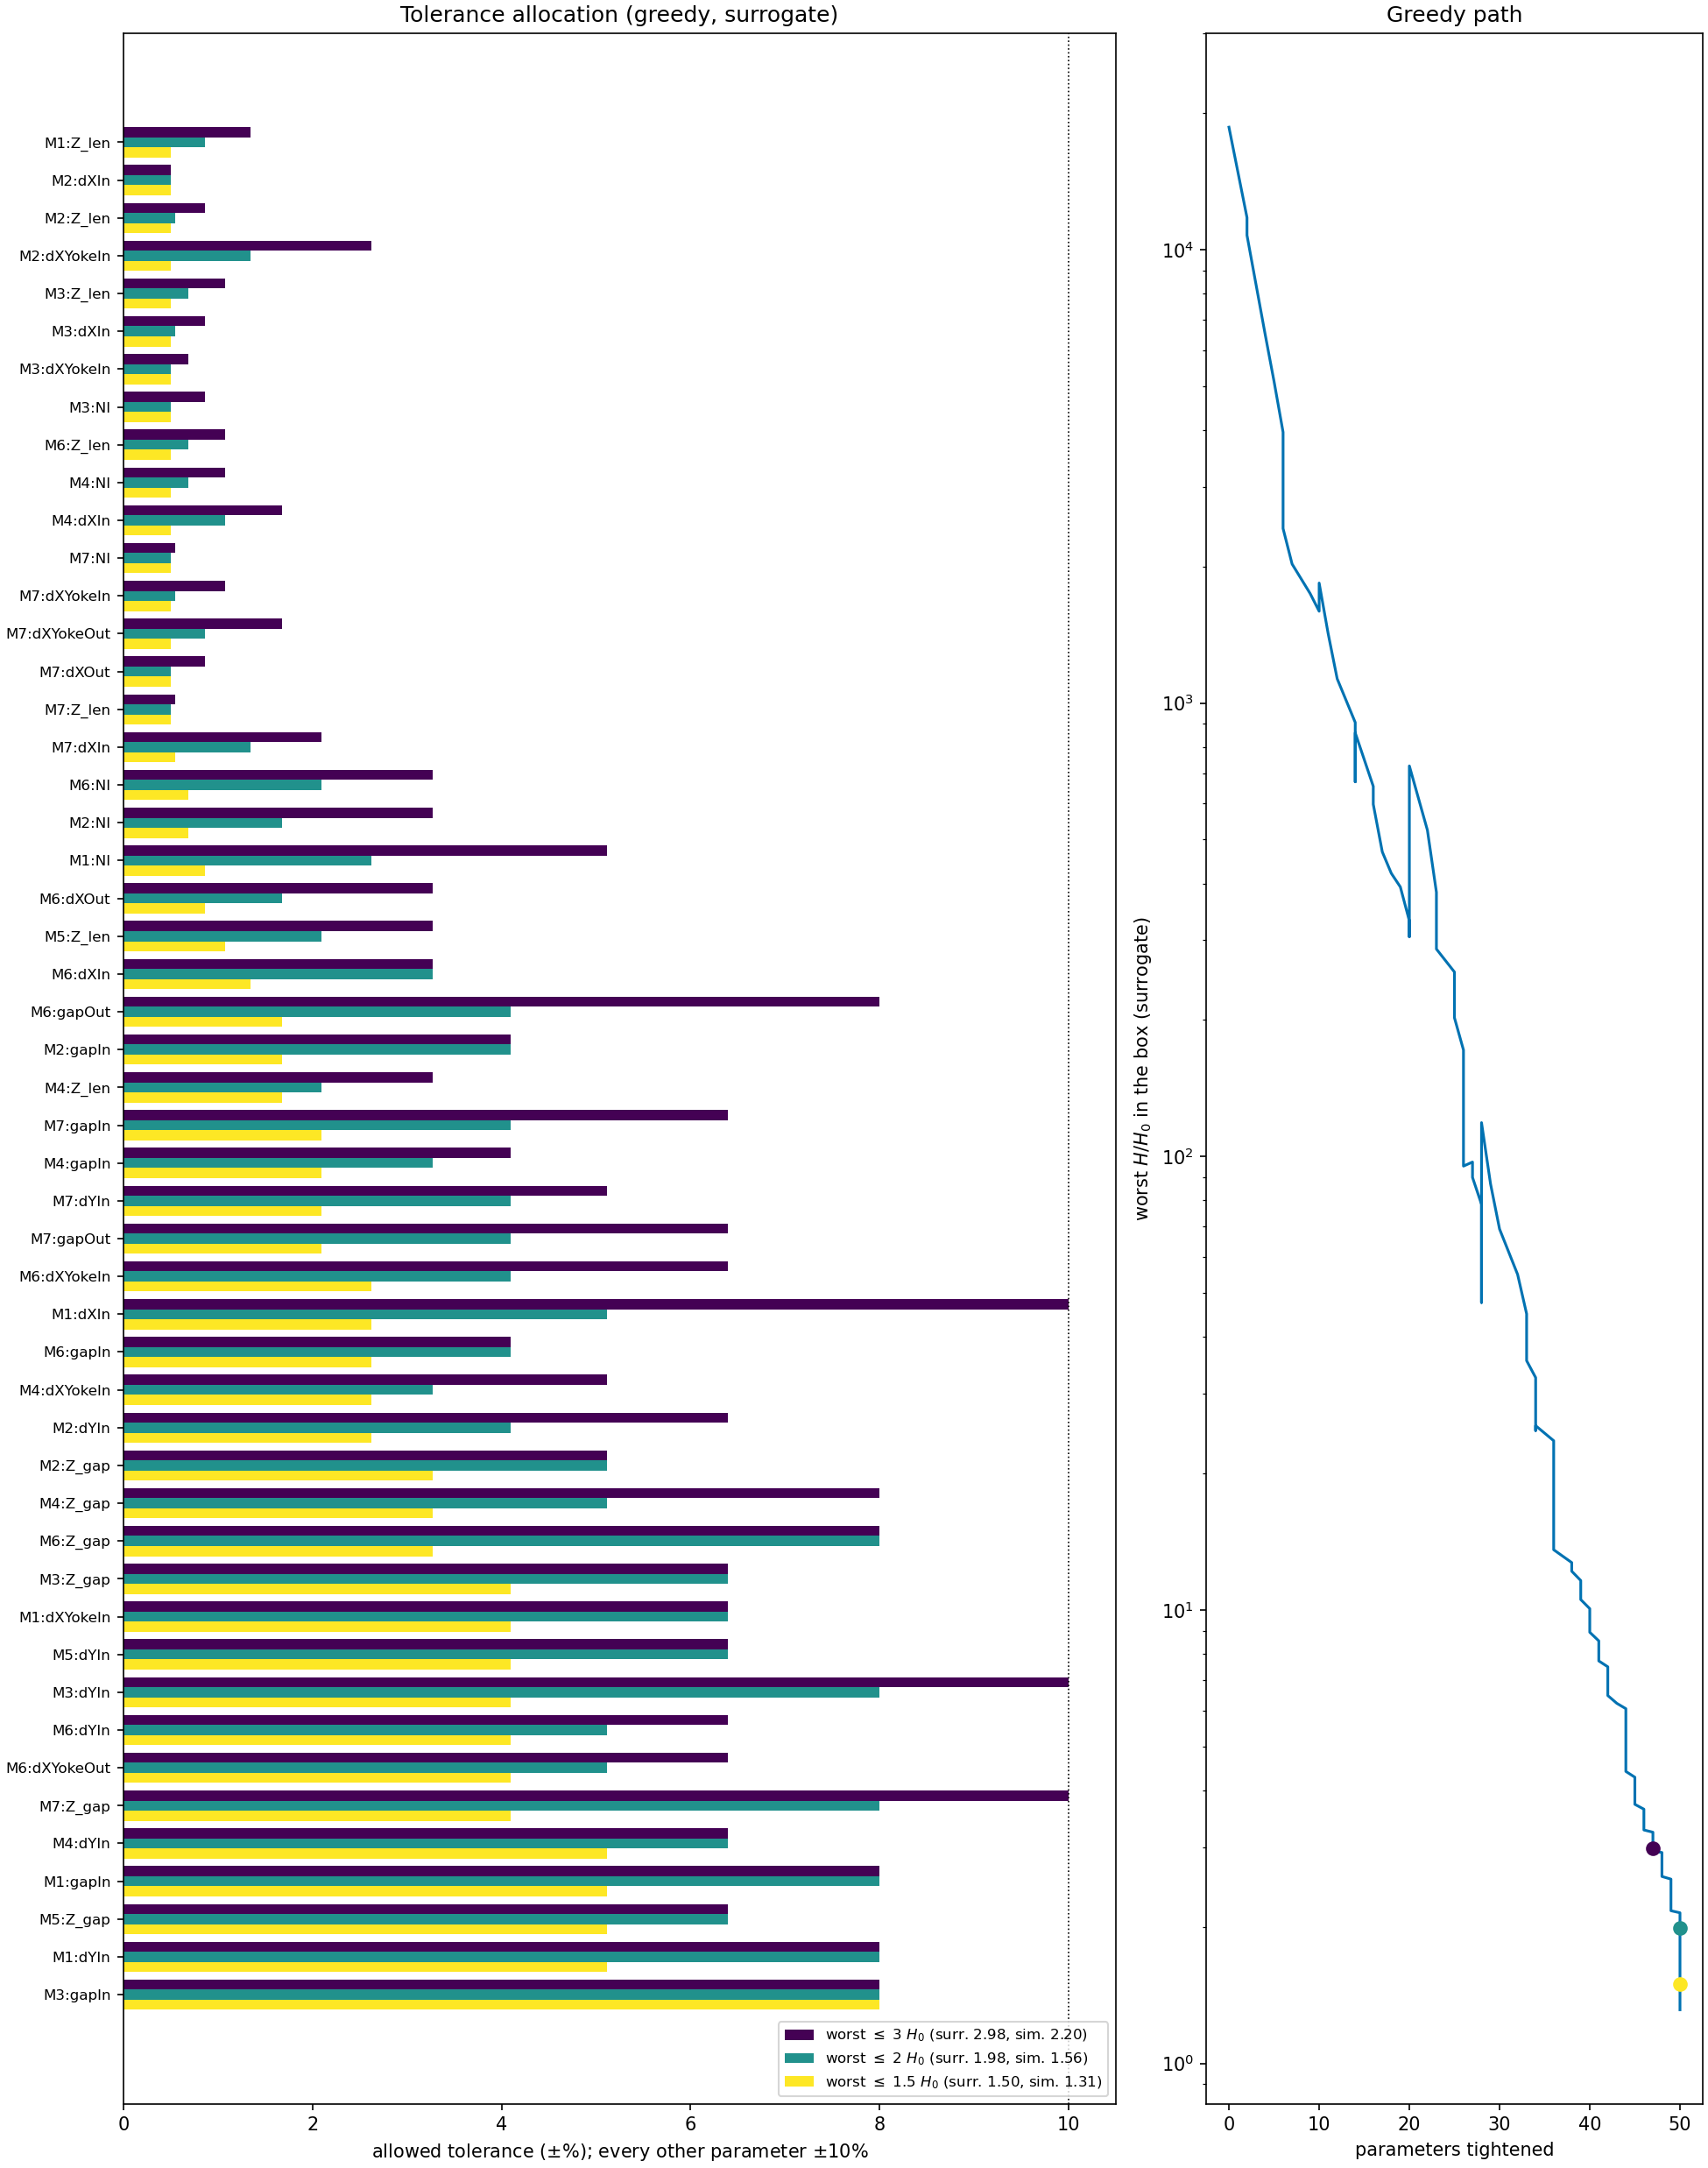
\includegraphics[width=\linewidth]{tolerance_allocation.png}
  \caption{Left: the tolerance allocations for a worst case of at most $3$, $2$ and $1.5\,H_0$
  (surrogate; simulated worst designs in the legend). Right: the greedy path, the worst case of
  the box against the number of parameters tightened.}
  \label{fig:allocation}
\end{figure}

\paragraph{Results} (Table~\ref{tab:allocation}, Fig.~\ref{fig:allocation}). A guarantee against
the worst case is demanding. For at most $\times3$, the allocation holds M2's entrance width to
$\pm0.5\%$ ($0.34$ cm), M7's field and length to $\pm0.55\%$ ($0.010$ T and $1.1$ cm) and M3's
inner yoke to $\pm0.7\%$; 15 parameters are below $\pm2\%$, three may stay at $\pm10\%$, and the
median tolerance is $4\%$. For at most $\times2$ it puts fourteen parameters below $\pm1\%$, six of
them at the $0.5\%$ floor, and for $\times1.5$ twenty-one, sixteen at the floor. The order follows
the sensitivities: M2's entrance, M7 (field, length, exit width, yokes) and M3 (inner yoke, field,
entrance) first, the gaps between magnets and the heights last. The simulated worst designs stay
below every target ($\times2.20$, $1.56$, $1.31$): at these small tolerances the surrogate is
conservative.

\subsection{Random tolerances}

Designs with every parameter independently uniform in $\pm2\%$, $\pm5\%$ and $\pm10\%$: eight of
each simulated, and 4096 per level from the surrogate (Fig.~\ref{fig:random}).
\begin{center}
\small
\begin{tabular}{lcccc}
\toprule
tolerance & simulated $\HH$ (8 designs) & surr.\ median & surr.\ 5--95\% & $P(H>H_0)$ \\
\midrule
$\pm2\%$  & 0.85, 0.91, 0.91, 1.00, 1.07, 1.09, 1.14, 1.15 & 1.02 & 0.86--1.29 & $57\%$ \\
$\pm5\%$  & 0.92, 0.93, 0.94, 1.17, 1.31, 1.44, 1.66, 1.76 & 1.17 & 0.81--2.21 & $73\%$ \\
$\pm10\%$ & 0.90, 1.88, 1.99, 2.30, 2.39, 3.93, 4.26, 11.3 & 2.05 & 0.89--10.2 & $91\%$ \\
\bottomrule
\end{tabular}
\end{center}
At $\pm2\%$ the hits stay within about $\pm15\%$. At $\pm5\%$ most designs stay within $\pm50\%$,
but the tail reaches $\times1.8$ among the simulated designs ($\times3.2$ at the surrogate's 99th
percentile). At $\pm10\%$ the median design is twice as bad and the tail reaches $\times11$ among
the simulated designs ($\times32$ at the surrogate's 99th percentile). The surrogate agrees with
the simulator design by design (median ratio simulator/surrogate $1.00$--$1.08$).

\begin{figure}[t]
  \centering
  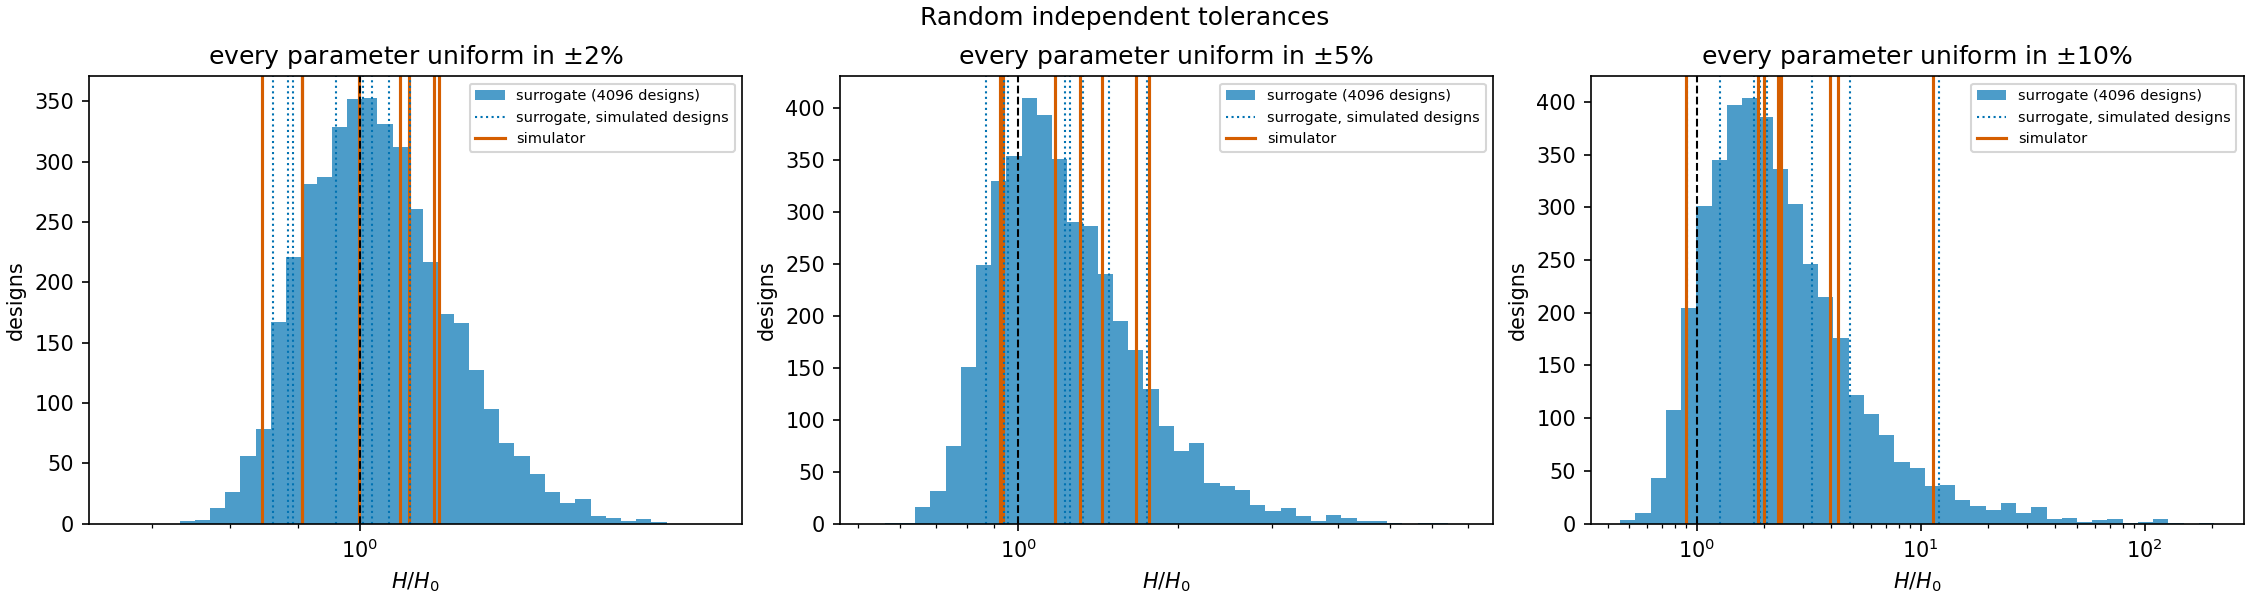
\includegraphics[width=\linewidth]{random_tolerances.png}
  \caption{Random independent tolerances: surrogate distribution of 4096 designs per level
  (histogram), and the eight simulated designs (solid: simulator, dotted: surrogate).}
  \label{fig:random}
\end{figure}

\subsection{Which muons respond}
\label{sec:momentum}

The muons are split into bins of $p_z$ (and separately $p_t$ and charge), and each bin's hits
$H_b$ get their own gradient, one-at-a-time effects and worst direction (Fig.~\ref{fig:pz_overview}).
Below $75$\,GeV the per-bin magnitudes carry the surrogate's larger uncertainty there
(Sec.~\ref{sec:validation}), so the directions and signs are the robust part; the simulated hits
per $p_z$ range (Fig.~\ref{fig:simpz}) confirm them.

\paragraph{Three populations.}
Half of the muons have $p_z<30$\,GeV, but at the nominal design the hits come from two groups
(Table~\ref{tab:pz}; simulated shares in parentheses): \emph{intermediate} momenta,
$30$--$75$\,GeV, with $67\%$ of the hits ($69\%$; $45\%$ at $40$--$50$\,GeV alone) at a hit rate
of $2\times10^{-6}$; and \emph{high} momenta above $125$\,GeV, $1.2\%$ of the muons but $25\%$ of
the hits ($23\%$ above $150$\,GeV), with hit rates up to $2\times10^{-3}$ above $300$\,GeV: the
muons the shield does not deflect enough. A third group, \emph{soft} muons of $20$--$30$\,GeV,
gives only $5\%$ of the hits but responds strongly to some changes. Compared with on-axis muons,
the production points raise the hits of every bin, most at $20$--$30$\,GeV ($\times2.0$),
$45$--$75$\,GeV ($+81\%$) and above $300$\,GeV ($+75\%$), least at $75$--$175$\,GeV
($+6$--$15\%$).

\begin{table}[t]
\centering
\caption{Per $p_z$ bin at the nominal design (surrogate): share of the muons and of the hits, hit
rate, relative sensitivity $|\nabla H_b|/H_b$ per tolerance unit, and the cosine between the
bin's gradient and that of the total.}
\label{tab:pz}
\begin{tabular}{lrrrrr}
\toprule
$p_z$ [GeV] & muons & share of hits & hit rate & $|\nabla H_b|/H_b$ & $\cos(g_b, g)$ \\
\midrule
10--20   & $1.7\%$   & $0.0\%$  & $1.3\times10^{-8}$ & 1.92 & $-0.40$ \\
20--30   & $48.4\%$  & $5.2\%$  & $1.3\times10^{-7}$ & 2.19 & $-0.55$ \\
30--45   & $28.8\%$  & $39.9\%$ & $1.7\times10^{-6}$ & 1.67 & $+0.96$ \\
45--75   & $15.3\%$  & $27.3\%$ & $2.2\times10^{-6}$ & 2.33 & $+0.90$ \\
75--125  & $4.7\%$   & $2.8\%$  & $7.6\times10^{-7}$ & 0.38 & $+0.31$ \\
125--175 & $0.89\%$  & $2.0\%$  & $2.9\times10^{-6}$ & 0.64 & $-0.10$ \\
175--225 & $0.23\%$  & $3.1\%$  & $1.7\times10^{-5}$ & 1.29 & $-0.15$ \\
225--300 & $0.08\%$  & $8.6\%$  & $1.4\times10^{-4}$ & 1.23 & $-0.16$ \\
$>300$   & $0.006\%$ & $11.0\%$ & $2.2\times10^{-3}$ & 2.55 & $-0.17$ \\
\bottomrule
\end{tabular}
\end{table}

\paragraph{The populations want opposite changes.}
The worst directions of the $30$--$45$ and $45$--$75$\,GeV bins agree ($\cos=0.98$), as do all
bins above $125$\,GeV ($0.96$--$1.00$), but the two groups are anti-aligned ($\cos=-0.37$ to
$-0.56$), and the soft bins are anti-aligned with the intermediate ones too (down to $-0.63$,
Fig.~\ref{fig:pz_alignment}). The total gradient, and every harmful direction of
Table~\ref{tab:walks}, follows the intermediate group ($\cos=0.90$--$0.96$). Simulated
(Fig.~\ref{fig:simpz}):
\begin{itemize}
  \item worst direction at $10\%$: the $40$--$50$\,GeV hits go from $538$ to $39\,759$ and the
        $50$--$60$\,GeV ones from $95$ to $17\,844$, while those above $150$\,GeV \emph{fall}
        from $270$ to $63$ and those below $30$\,GeV from $48$ to $8$;
  \item opposite direction: the $40$--$50$\,GeV hits fall from $538$ to $87$, but those of
        $20$--$30$\,GeV rise from $48$ to $1241$ and those above $150$\,GeV from $270$ to $1753$;
  \item the box corner of the walks: only $30$--$75$\,GeV ($819\to1\,374\,628$), the
        high-momentum hits fall ($270\to63$);
  \item random $\pm10\%$ designs can open any group: the worst of the eight ($\times11$) raises
        the $40$--$50$\,GeV hits from $538$ to $8633$, another ($\times0.9$ in total) those above
        $150$\,GeV from $270$ to $555$ while the $40$--$50$\,GeV ones fall to $181$, and another
        ($\times3.9$) both the soft ($48\to2491$) and the high-momentum ($270\to890$) ones.
\end{itemize}

\paragraph{Which parameters act on which muons} (Fig.~\ref{fig:pz_sensitivity}).
The high-momentum hits are controlled by the \emph{upstream} magnets: the lengths and fields of
M1--M4, each changing the hits above $175$\,GeV by $40$--$160\%$ at its worse limit. The
intermediate hits are controlled by the entrance width of M2 ($+170$--$240\%$ at the worse
limit), the inner yoke of M3, and the \emph{downstream} magnet M7 (its field: $+126$--$159\%$ of
the $30$--$75$\,GeV hits). The soft hits respond most to the entrance widths of M2 and M3 and the
inner yoke of M3 (up to $\times5.6$). This explains \texttt{act1}: changing M1--M4 together shifts
hits between the high-momentum group and the others, and the nominal design balances them.

\paragraph{Transverse momentum and charge.}
The sensitivity grows with $p_t$ up to $1.5$\,GeV ($0.97$ to $1.58$ per tolerance unit) and the
neighbouring $p_t$ bins want the same changes ($\cos\ge0.92$), the extreme ones less ($0.69$,
Fig.~\ref{fig:pt}). The muons above $1.5$\,GeV ($1.6\%$ of the muons, $28\%$ of the hits) are less
sensitive ($0.97$) and aligned with the rest at $\cos=0.69$--$0.92$. Positive muons give $61\%$ of
the hits; both charges respond to the same changes ($\cos=0.98$), the $\mu^-$ somewhat more
strongly ($1.24$ vs.\ $0.98$).

\begin{figure}[t]
  \centering
  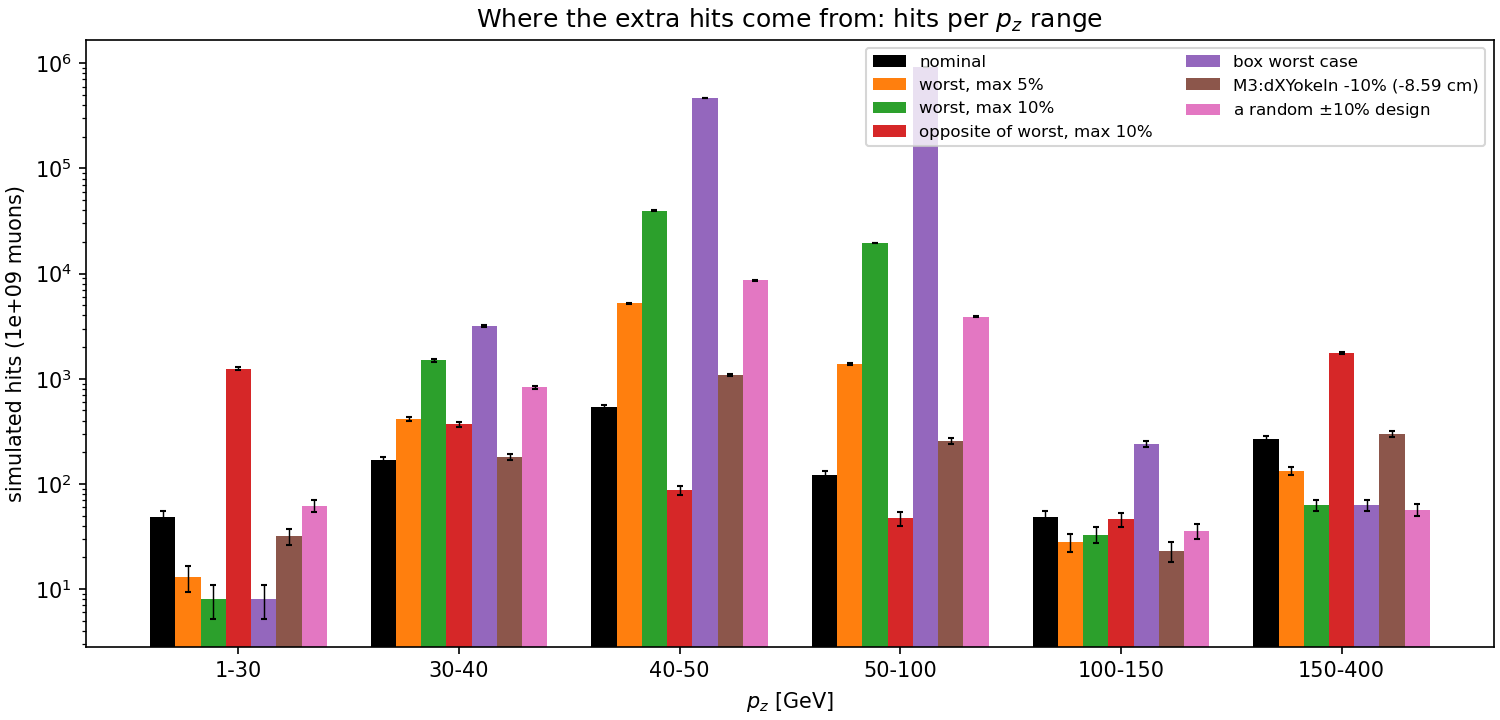
\includegraphics[width=\linewidth]{sim_pz_profiles.png}
  \caption{Simulated hits per $p_z$ range for the nominal design and some designs of
  Table~\ref{tab:concrete}.}
  \label{fig:simpz}
\end{figure}

\begin{figure}[t]
  \centering
  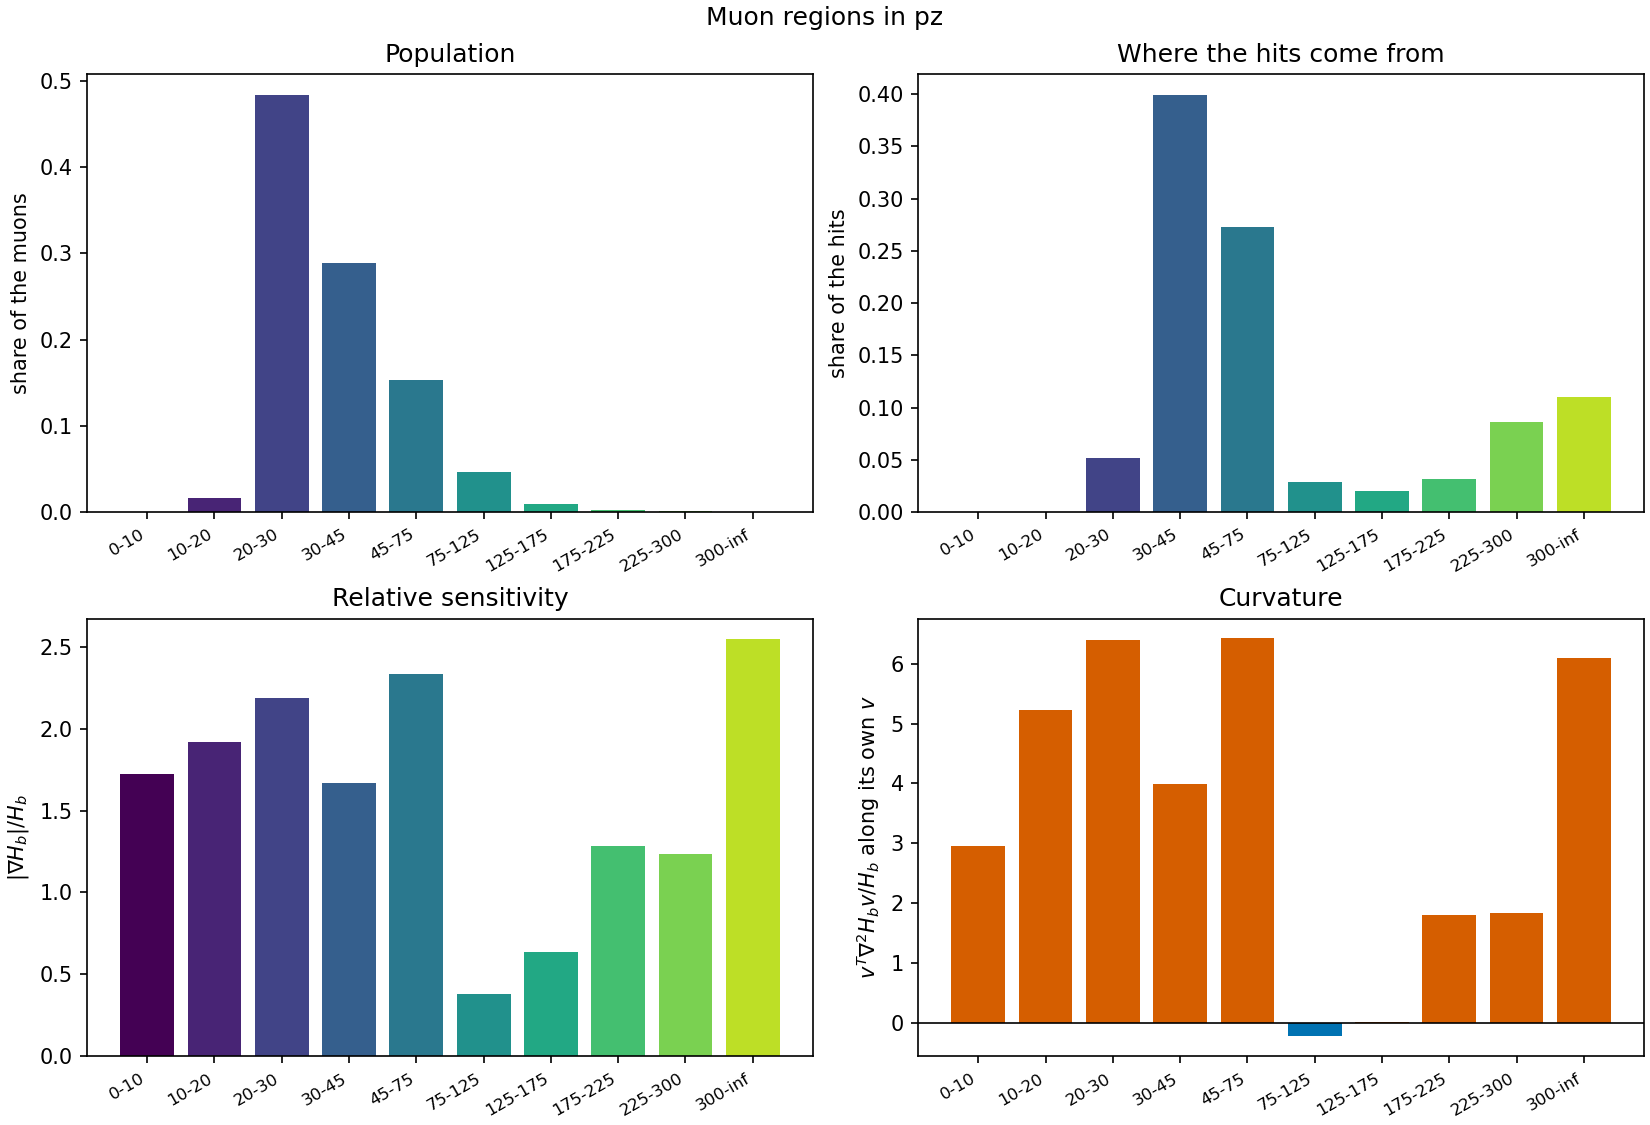
\includegraphics[width=0.9\linewidth]{pz_bins_overview.png}
  \caption{Per $p_z$ bin (surrogate): share of the muons and of the hits, relative sensitivity
  and curvature along the bin's own worst direction.}
  \label{fig:pz_overview}
\end{figure}

\begin{figure}[t]
  \centering
  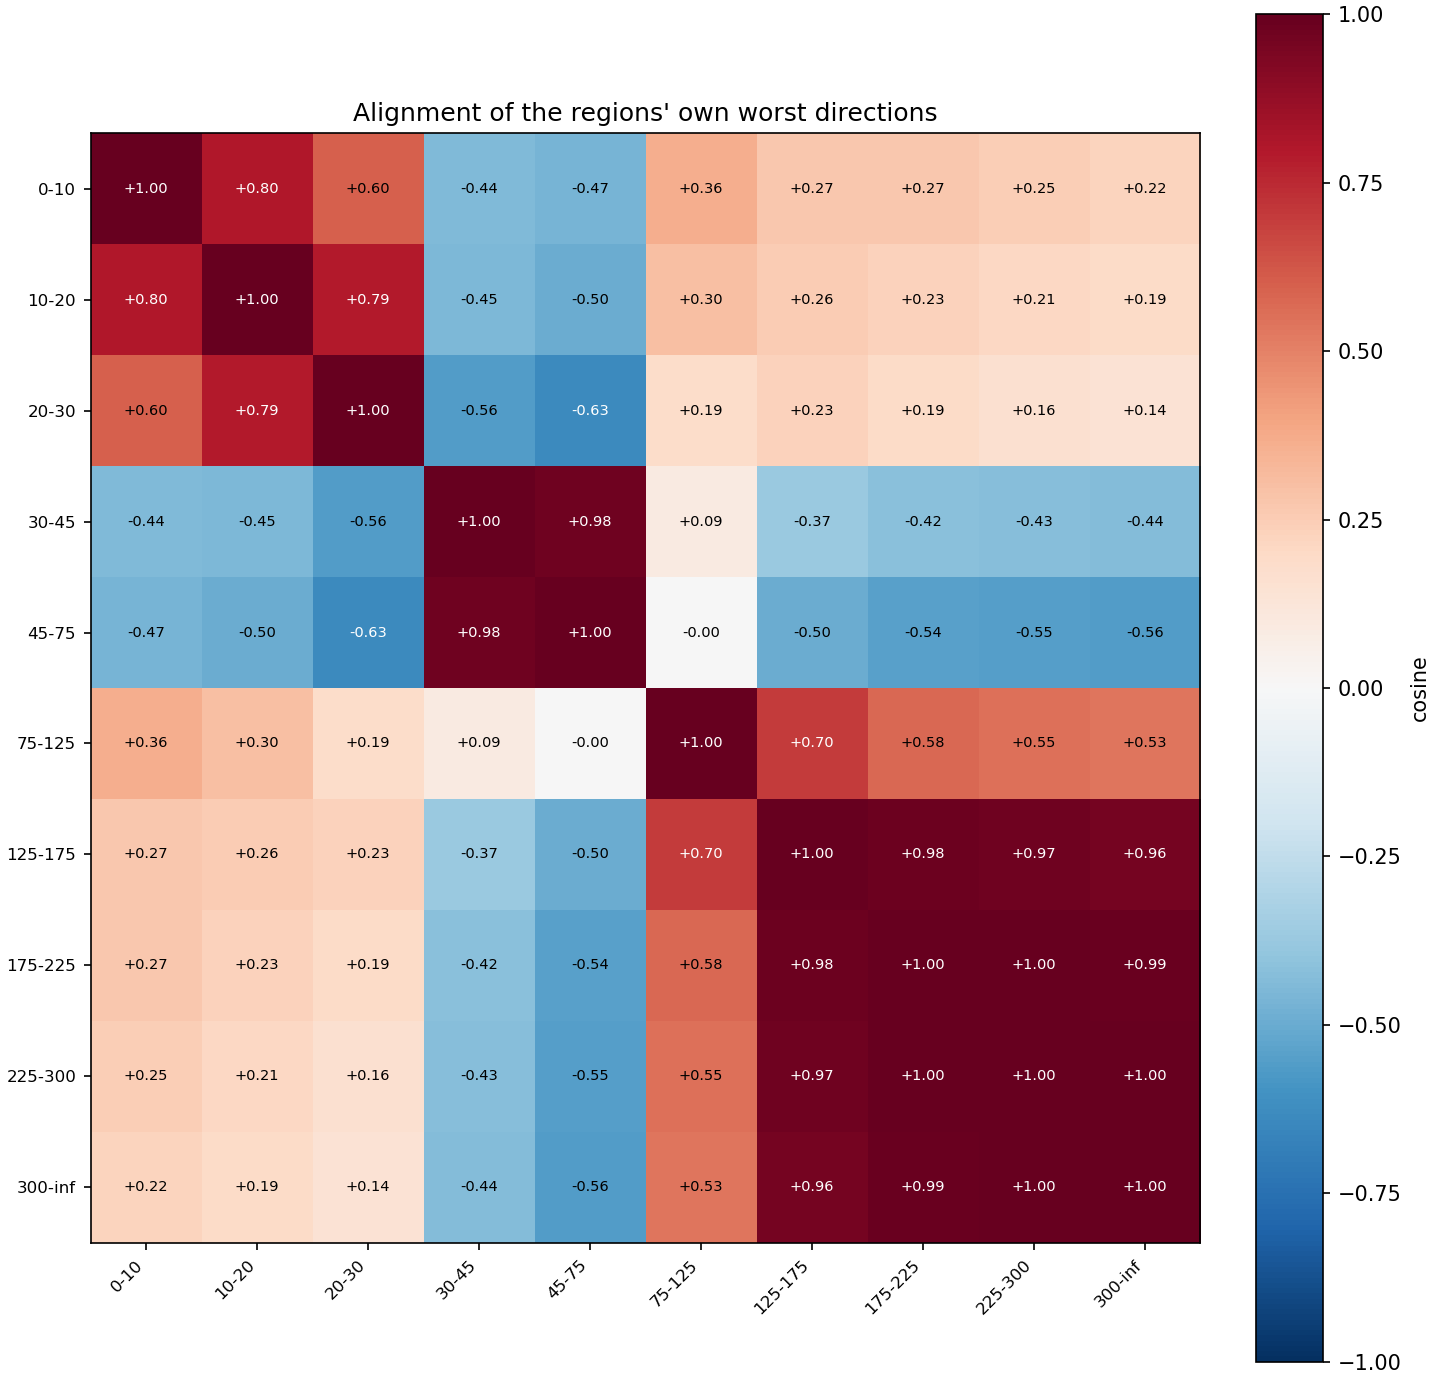
\includegraphics[width=0.62\linewidth]{pz_bins_alignment.png}
  \caption{Cosine between the worst directions of the $p_z$ bins: the intermediate momenta
  ($30$--$75$\,GeV) want the opposite changes to the high ($>125$\,GeV) and the soft
  ($10$--$30$\,GeV) ones.}
  \label{fig:pz_alignment}
\end{figure}

\begin{figure}[p]
  \centering
  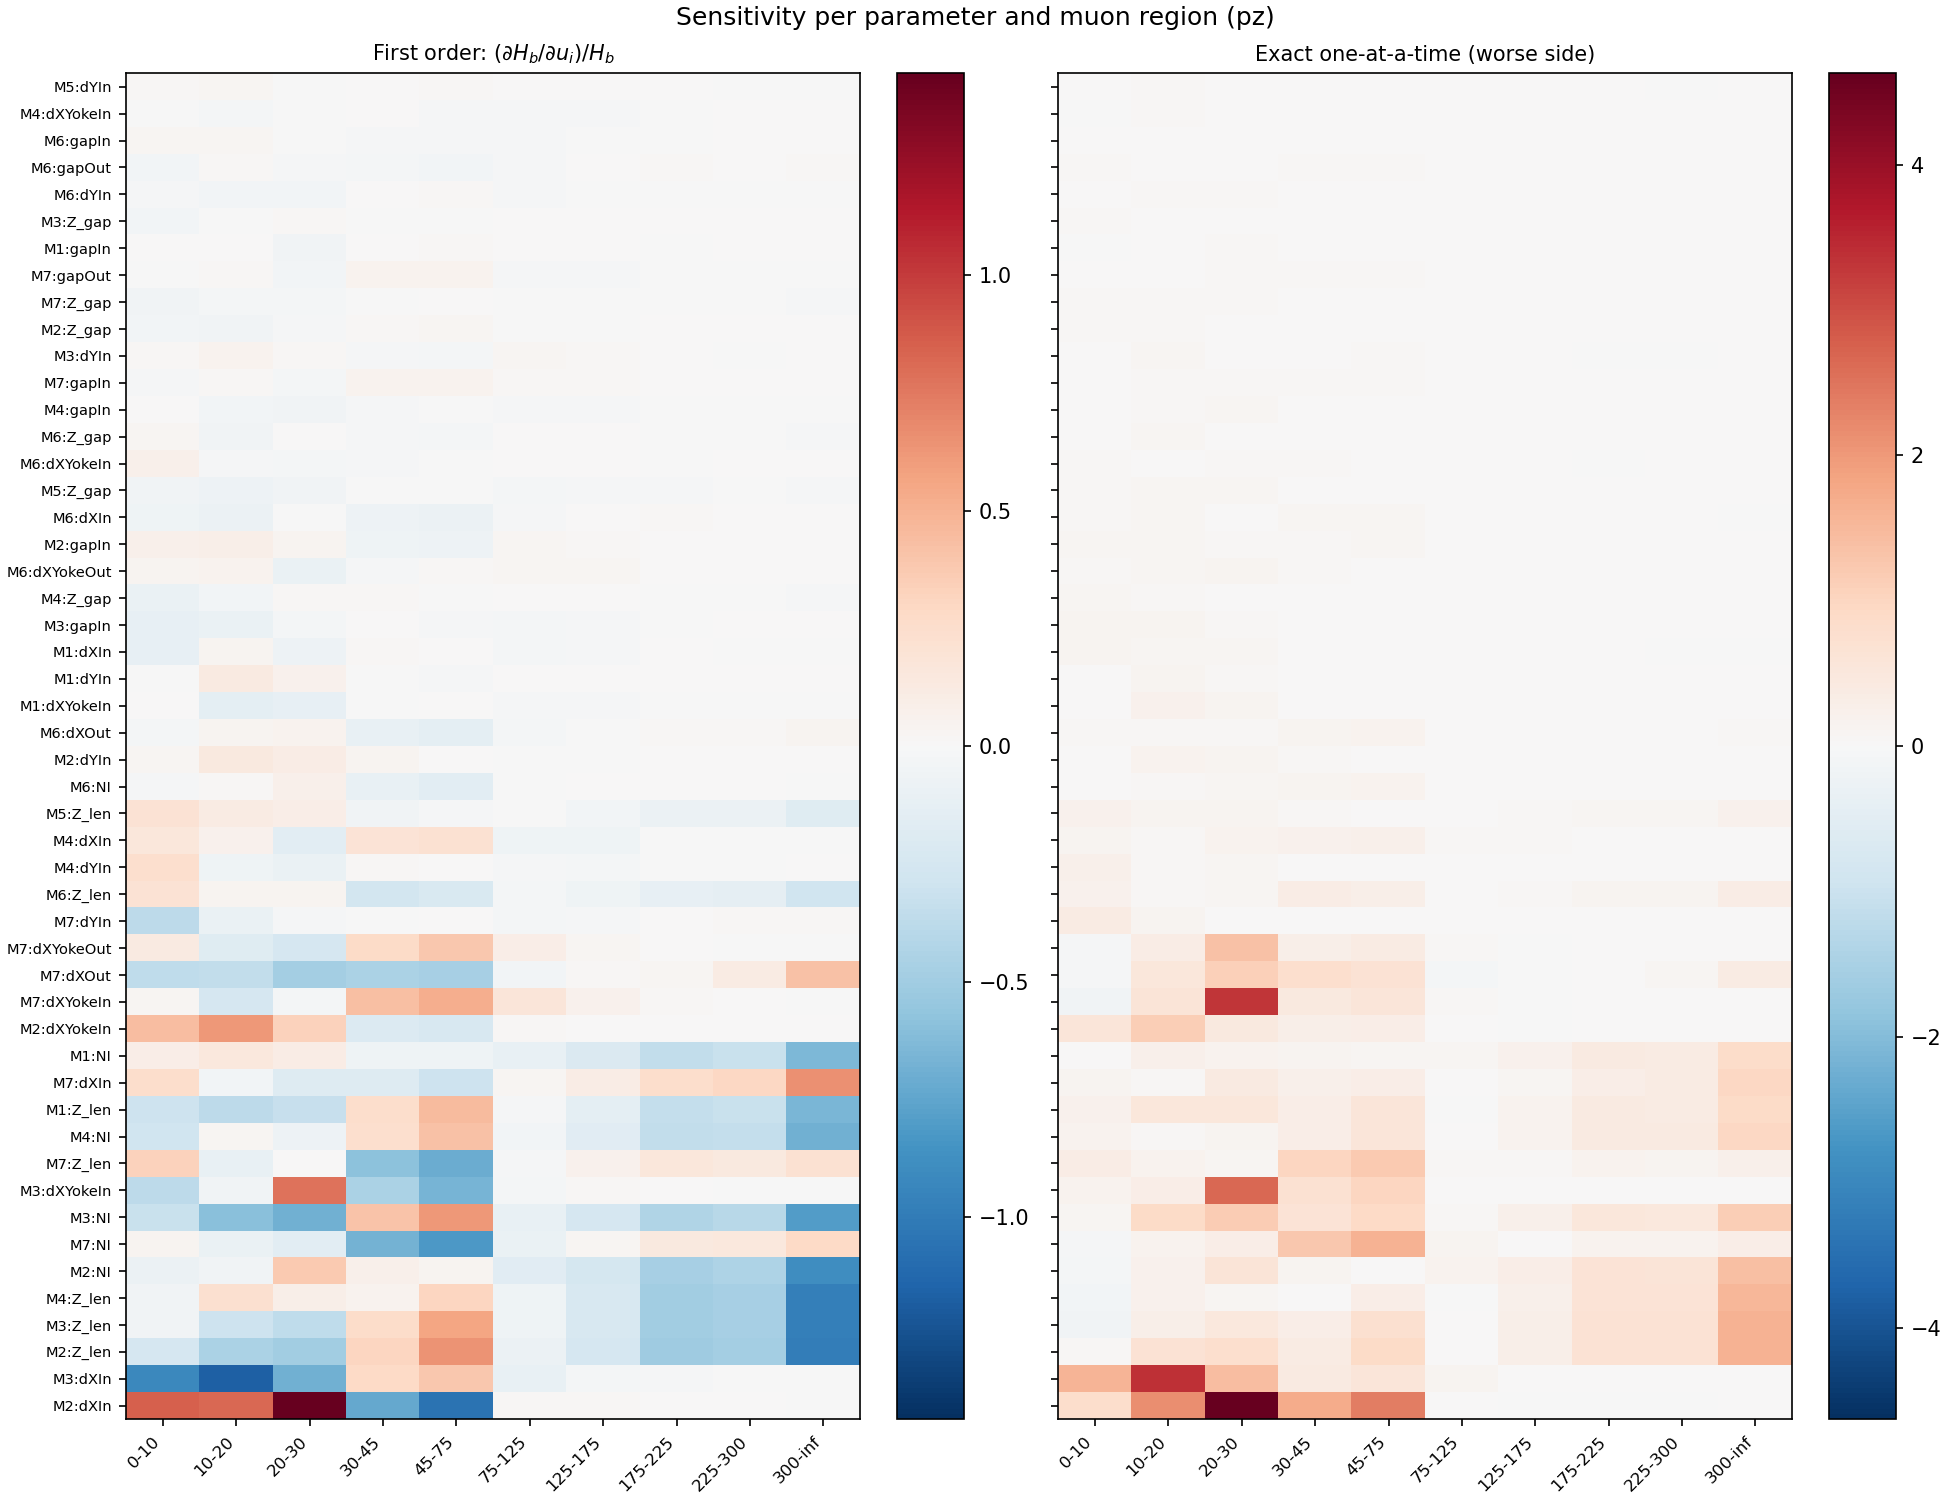
\includegraphics[width=\linewidth]{pz_bins_sensitivity.png}
  \caption{Sensitivity of each $p_z$ bin to each parameter, relative to the bin's own hits.
  Left: first order. Right: exact one-at-a-time change at the worse of $\pm10\%$.}
  \label{fig:pz_sensitivity}
\end{figure}

\begin{figure}[t]
  \centering
  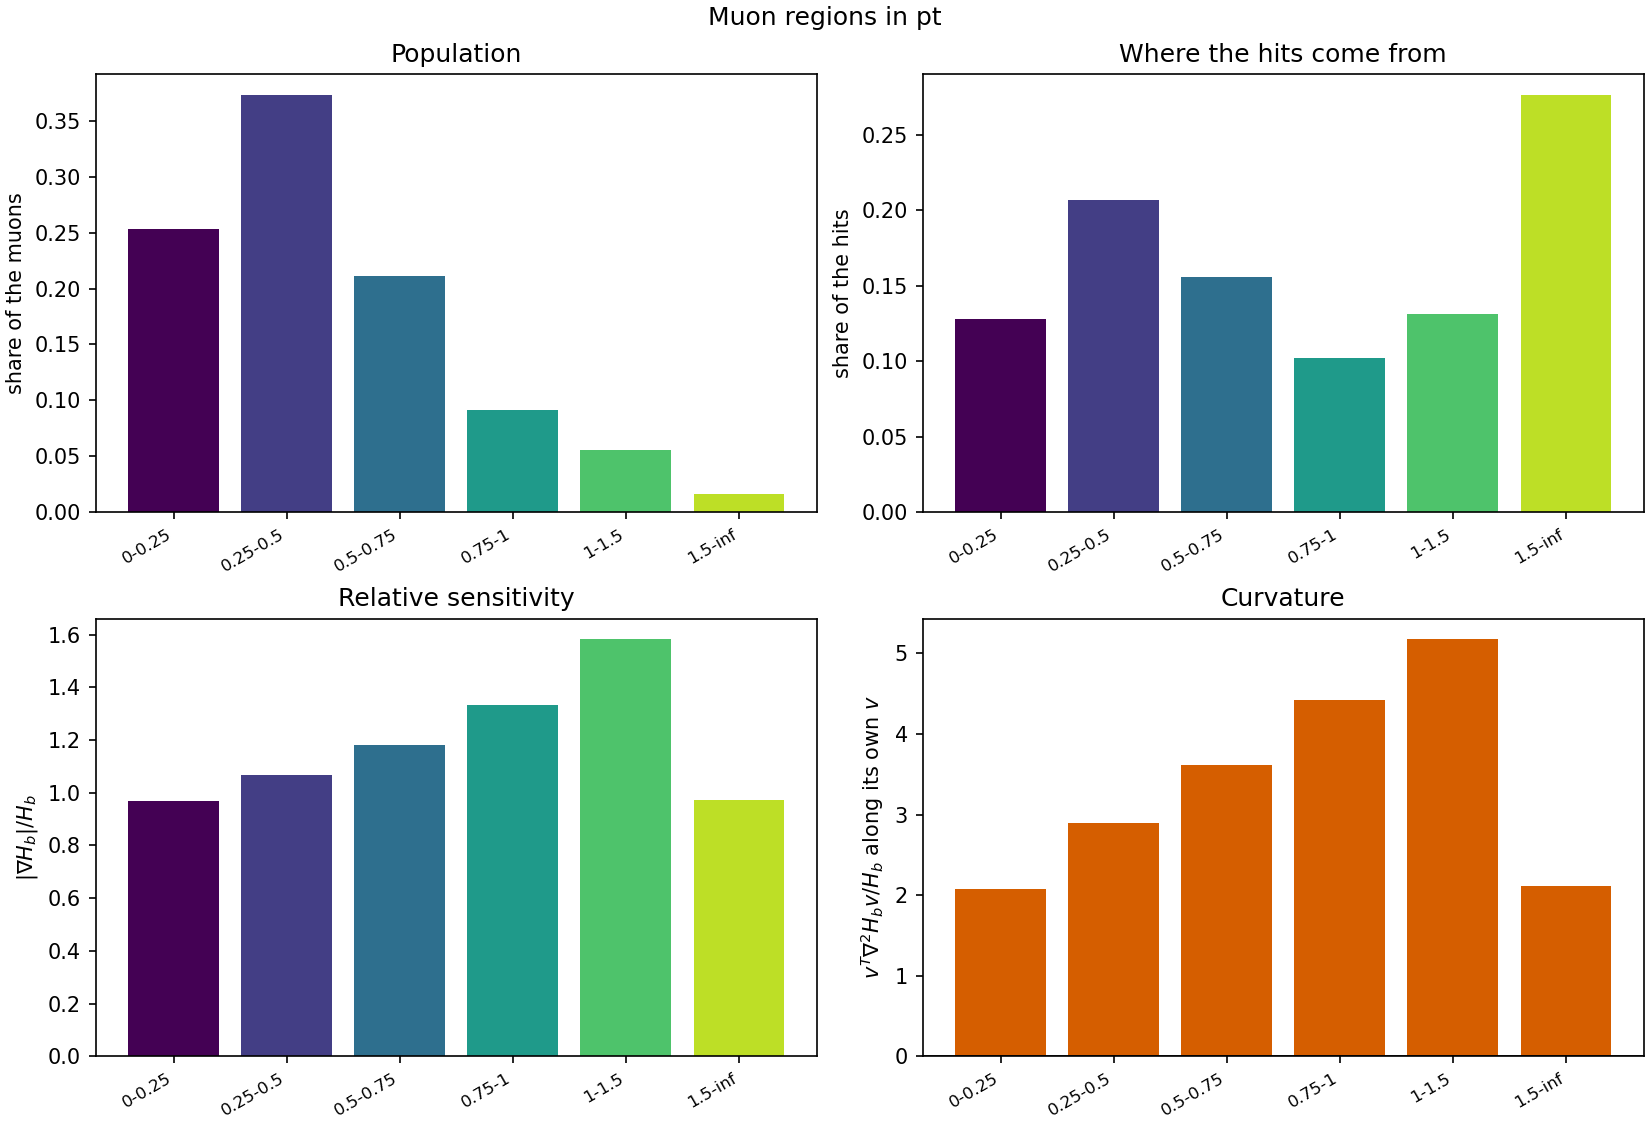
\includegraphics[width=0.49\linewidth]{pt_bins_overview.png}\hfill
  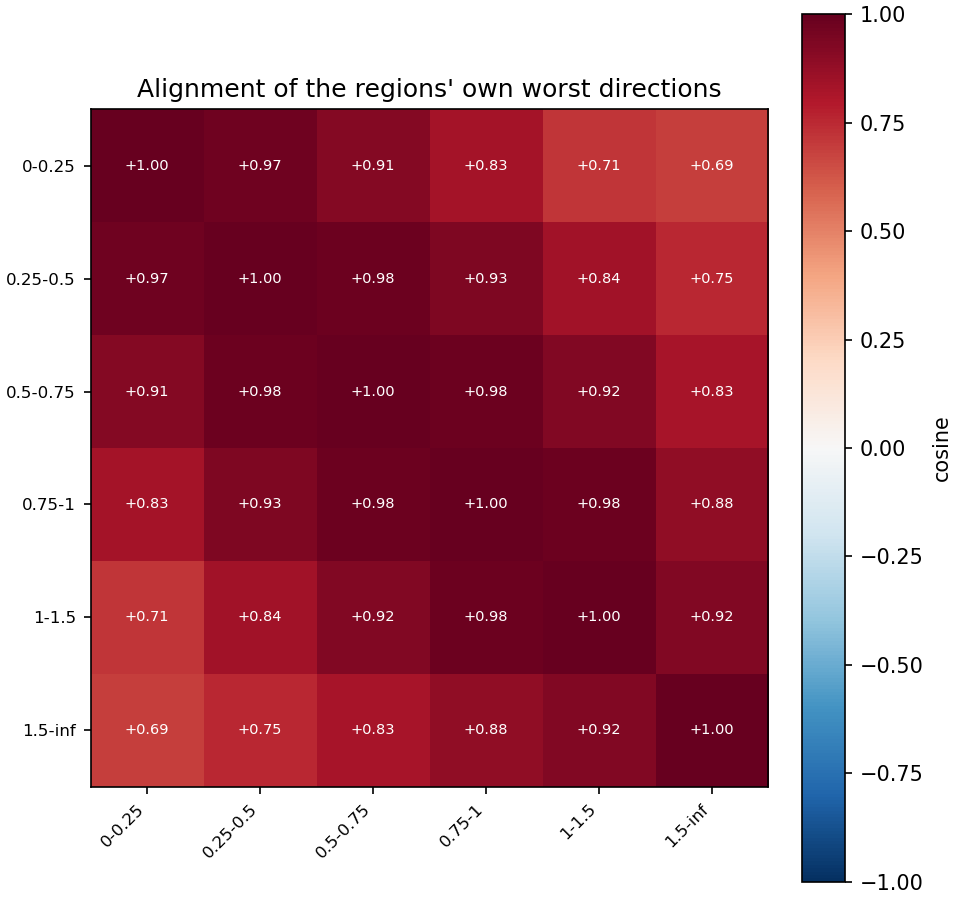
\includegraphics[width=0.42\linewidth]{pt_bins_alignment.png}
  \caption{Per $p_t$ bin: overview (left) and alignment of the bins' worst directions (right).}
  \label{fig:pt}
\end{figure}

\clearpage
%==============================================================================
\section{Conclusions}
%==============================================================================

\begin{enumerate}
  \item \textbf{The design is fragile to coordinated deviations.} With every parameter off by up
        to $\varepsilon$, the worst design found (on the surrogate, then simulated) gives
        $\times1.7$ at $\varepsilon=1\%$, $\times3.9$ at $2\%$, $\times9.7$ at $3\%$, $\times121$
        at $5\%$ and $\times2840$ at $10\%$; these are lower bounds on the true worst case, tight
        up to $3\%$. Moving every parameter by $1.4\%$ with the sign of its gradient already
        gives $\times2.5$.
  \item \textbf{Bounding the worst case needs sub-percent tolerances on a few parameters and a
        few percent on most.} The allocation found for at most $\times3$ holds M2's entrance
        width to $\pm0.5\%$, M7's field and length to $\pm0.55\%$ and M3's inner yoke to
        $\pm0.7\%$, 15 parameters below $\pm2\%$, median $4\%$; for at most $\times2$, fourteen
        below $\pm1\%$ (simulated $\times2.20$ and $\times1.56$). M2, M7 and M3 need the tightest
        tolerances, the gaps between magnets and the heights the loosest.
  \item \textbf{Single parameters underestimate the risk.} The worst one at its $\pm10\%$ limit
        (the entrance width of M2) gives $\times2.6$; the field, length and exit width of M7
        give $\times1.7$--$2.1$. The top three changes of the worst direction together give
        $\times6$, the top ten $\times30$: the factors multiply. M7 matters most, then M2, M3 and
        M6; the magnet heights hardly matter ($\le3\%$ each at $\pm10\%$).
  \item \textbf{Random deviations are much milder than the worst case.} Independent errors of
        $\pm2\%$ keep the hits within about $\pm15\%$; at $\pm5\%$ most designs stay within
        $\pm50\%$, with a tail to $\times2$--$3$; at $\pm10\%$ the median design is twice as bad
        and the tail reaches $\times11$--$32$. A specification can therefore be much looser if the
        errors are independent than if it must hold against the worst combination.
  \item \textbf{Different muons pull in opposite directions.} The hits come from muons of
        $30$--$75$\,GeV ($67\%$) and above $125$\,GeV ($25\%$). Every harmful direction near the
        nominal design acts through the first group, while the high-momentum hits fall; the
        reverse direction raises the soft and high-momentum hits instead. The dominant
        active-subspace direction (the lengths and fields of M1--M4) trades hits between the
        groups and is harmful on both sides.
  \item \textbf{The surrogate is quantitative within the tolerance region.} It reproduces the
        one-at-a-time effects to $3\%$, the walks within one tolerance unit to $1$--$2\sigma$, the
        reference designs in the box to $6\%$ and the worst designs within $\pm1$--$3\%$ to
        $8$--$13\%$ (conservatively). It overestimates the worst designs at $\pm5\%$ ($\times1.8$)
        and $\pm10\%$ ($\times7$), so every number used for a decision here is simulated.
  \item \textbf{The production points matter for the level, not the conclusions.} Starting the
        muons where they are produced instead of on axis raises the nominal hits by about half,
        and makes M2's entrance width slightly more critical than M7's field; the directions,
        the mechanisms and the tolerances are those of the on-axis analysis.
\end{enumerate}

\section*{Limitations}
\begin{itemize}
  \item Uniform fields per magnet block, no field maps. The height of a magnet moves its entrance
        and exit together.
  \item Muons come from the generative flow, so the absolute numbers depend on how well the flow
        reproduces the muon spectrum and the production points.
  \item A third of the training designs come from the first analysis (on-axis muons, nominal
        heights); the model learns the production point and the heights from the rest.
  \item The surrogate's errors are the scatter of its members: they miss a bias the members
        share, such as the one far from the nominal design (Sec.~\ref{sec:validation}). Only the
        top Hessian eigenvector is clearly separated.
  \item The random-tolerance distributions rest on eight simulated designs per level and on the
        surrogate for their tails.
  \item The worst designs within a tolerance are found on the surrogate: their simulated values
        bound the true worst case from below, tightly up to $\pm3\%$, possibly loosely at $\pm5\%$
        and $\pm10\%$, where the surrogate is unreliable. The tolerance allocation is a greedy
        heuristic, not an optimum.
\end{itemize}

\clearpage
\appendix
\section{Free parameters}
\begin{table}[h]
\centering
\caption{Free parameters and nominal values (lengths in cm, $B$ in T). \texttt{dYIn} is the
height; the exit height \texttt{dYOut} is set equal to it.}
\label{tab:params}
\small
\setlength{\tabcolsep}{4pt}
\begin{tabular}{lrrrrrrrrrr}
\toprule
magnet & \texttt{Z\_gap} & \texttt{Z\_len} & \texttt{dXIn} & \texttt{dXOut} & \texttt{dYIn} & \texttt{gapIn} & \texttt{gapOut} & \texttt{dXYokeIn} & \texttt{dXYokeOut} & $B$ \\
\midrule
M1 &  --   & 151.5 & 63.12 & --    & 10.0  & 8.149 & --    & 64.12 & --     & 1.9 \\
M2 & 15.0  & 224.9 & 68.04 & --    & 10.0  & 8.431 & --    & 70.62 & --     & 1.9 \\
M3 & 16.12 & 225.0 & 64.81 & --    & 13.93 & 8.986 & --    & 85.88 & --     & 1.9 \\
M4 & 15.0  & 224.0 & 39.02 & --    & 11.08 & 8.327 & --    & 97.53 & --     & 1.9 \\
M5 & 15.0  & 120.4 & --    & --    & 30.0  & --    & --    & --    & --     & -- \\
M6 & 15.0  & 168.0 & 20.0  & 30.0  & 40.0  & 24.92 & 9.388 & 97.18 & 102.7  & $-1.2$ \\
M7 & 15.0  & 193.1 & 37.95 & 67.81 & 47.77 & 8.000 & 8.000 & 124.8 & 94.92  & $-1.9$ \\
\bottomrule
\end{tabular}
\end{table}

\section{Integrating the surrogate over the muons}
\label{app:quadrature}

With $A(z)$ the kinematic envelope of the sampled muons and $N=10^9$,
\begin{equation}
  H(u) = \frac{N}{\int\!\mathrm{d}^2z\,\mathcal{N}(z)A(z)}\sum_{q=\pm1}P(q)\int\!\mathrm{d}^2z\,
  \mathcal{N}(z)\,A(z)\int_0^{2\pi}\!\frac{\mathrm{d}\varphi}{2\pi}\,
  \mathbb{E}_{r\mid z,q}\,p\big(\text{hit}\mid u, x(z,\varphi,q,r)\big),
\end{equation}
where $z$ is the flow's 2-d momentum latent, $\varphi$ the azimuth (uniform), $q$ the charge (with
the data's $\mu^+$ fraction) and $r$ the production point, which the flow draws given the
momentum and charge. The momentum, azimuth and charge are integrated on a grid: $801^2$ latent
points on $[-7,7]^2$ with Gaussian weights, 64 azimuths and both charges for the derivatives;
$201^2\times64\times2$ points, with the trunk features cached, for everything else. The
production point is drawn once per grid node from a fixed seed, so the grid is a fixed set of
muons; these draws are its only noise.

Against a reference grid of $1601^2\times64\times2$ nodes with four production points each
(Fig.~\ref{fig:quadrature}), the derivative grid is off by $4\times10^{-4}$ in $H$,
$1.6\times10^{-3}$ in the gradient and $1.3\times10^{-3}$ in the Hessian, and the cached grid by
$2.5\times10^{-3}$, $5.6\times10^{-3}$ and $4.2\times10^{-3}$ (rms over eight position seeds); four
production points per node would halve the cached grid's errors. $10^9$ sampled muons scatter by
$0.7\%$ in $H_0$ and $2\%$ above $300$\,GeV, and $10^8$ by $3\%$ in $H$, gradient and Hessian
alike. With on-axis muons (the first analysis) the grid was exact to $10^{-5}$, and quasi-Monte
Carlo helped sampling only by a factor two. Importance-sampling the simulator at a raised
temperature does not help either: the hits that matter are at intermediate momenta, of which a
hotter sample holds fewer.

\begin{figure}[h]
  \centering
  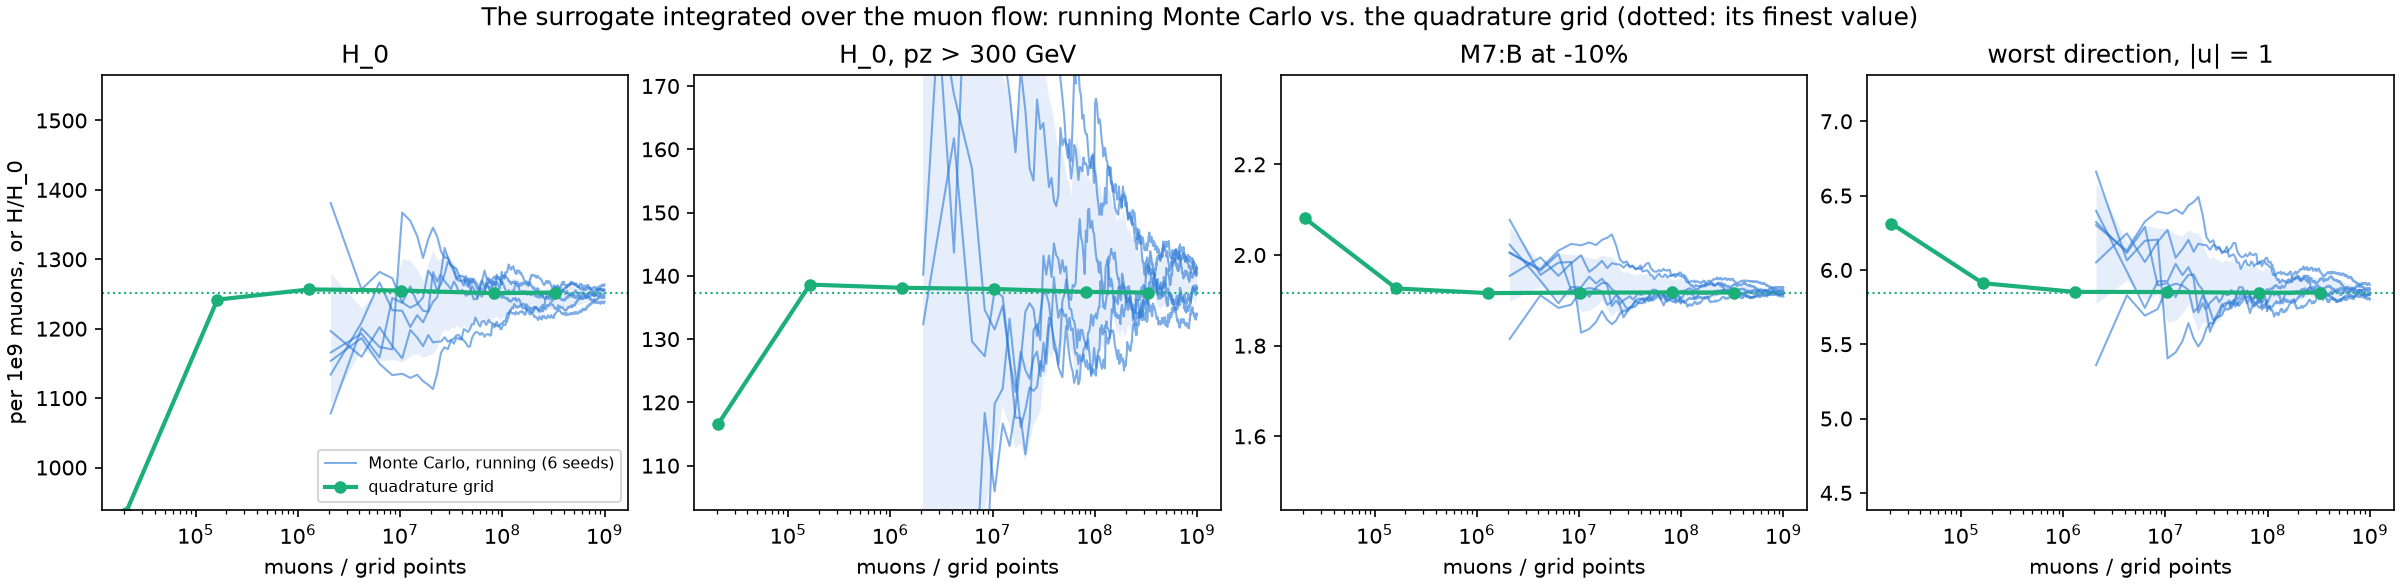
\includegraphics[width=\linewidth]{quadrature_convergence.png}\\[1ex]
  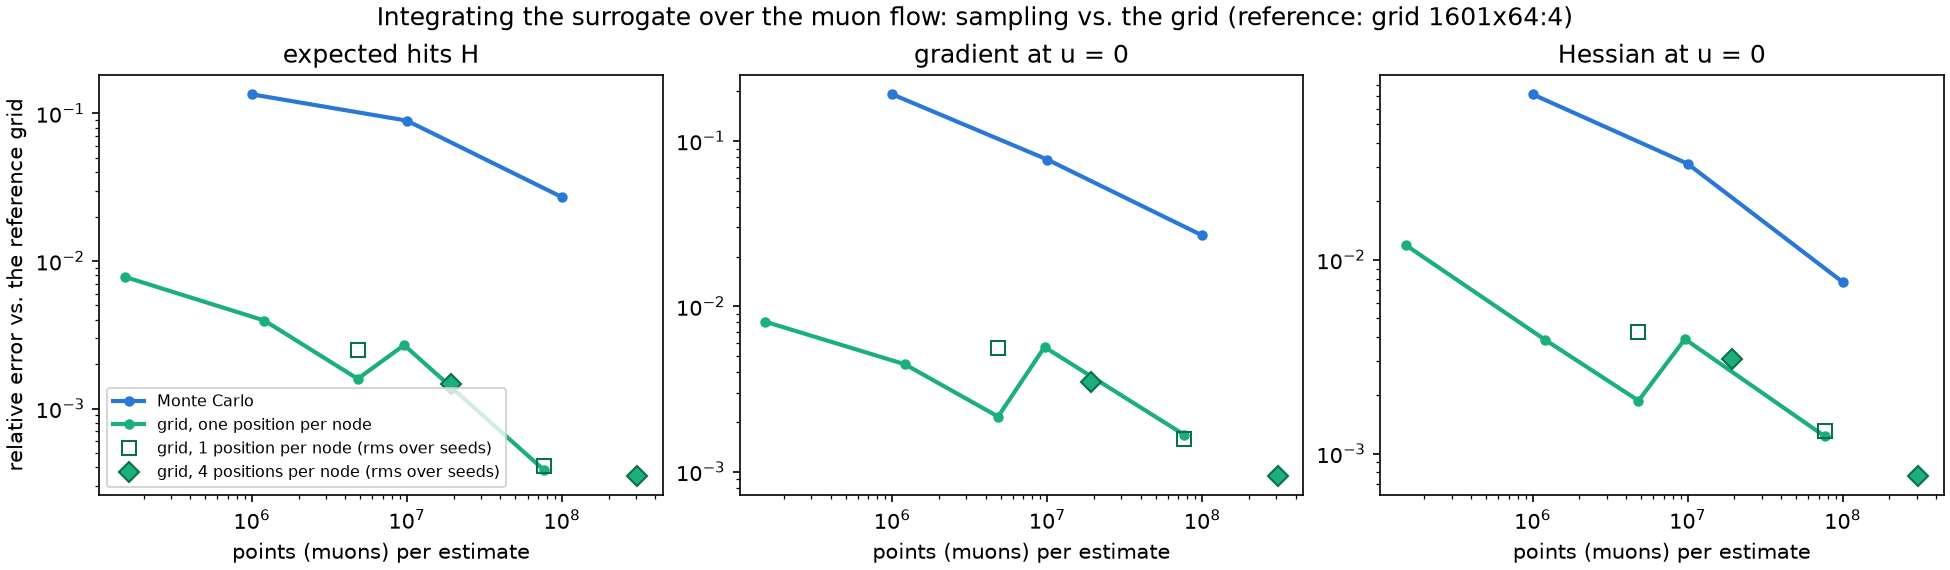
\includegraphics[width=0.85\linewidth]{quadrature.png}
  \caption{Top: Monte Carlo estimates (six seeds) against the grid at increasing resolution, for
  the nominal hits, the hits above $300$\,GeV, the field of M7 at $-10\%$ and one tolerance unit
  along the worst direction. Bottom: relative error against the reference grid, for Monte Carlo
  (rms over eight seeds) and the grid with one production point per node; squares and diamonds:
  the grids of the analysis with one and four production points per node, rms over eight
  position seeds.}
  \label{fig:quadrature}
\end{figure}

\section{How the surrogate was chosen}
\label{app:study}

The choices come from a study of the surrogates (\texttt{experiments/}) made for the first
analysis (43 parameters, muons on axis) and not repeated here: this analysis uses the settings it
found best. The study used four toy problems with exact answers (a binary outcome per sample with
known probability; 10--43 parameters) and the shield against its reference designs
(Fig.~\ref{fig:study}).
\begin{itemize}
  \item \textbf{Modelling each muon is what makes it work.} A response surface fitted to the same
        simulations without the muons needs about ten times more simulation for the same gradient.
  \item \textbf{Training data.} Many designs with few muons each beat few designs with many; all
        designs at once beat a rolling buffer; the designs must cover the region where the
        derivatives are read. A hotter momentum temperature ($T=2$) is much better than $T=1$ or
        $1.5$, and $T=3$ no better than $T=2$. A tailored training proposal (the provably best one
        for the error on $H$) would give at most $1.7\times$ the effective training muons of
        $T=2$, so the temperature is kept. Adding designs far from the nominal one helped only
        with an adaptive pool: a pool uniform in the box alone did not lower the box error on the
        nominal muons, with the adaptive pool it fell by a fifth (four seeds each, scored on the
        same references). This analysis therefore uses many $T=2$ designs with $10^6$ muons each,
        a wider pool instead of the uniform one, and an adaptive pool.
  \item \textbf{Architecture.} The DeepONet is the most reliable for the hit rate. At the final
        scale ($2\times10^8$ rows) capacity matters (128 units, 32 features), and averaging seeds
        removes most of the scatter of the gradient. Reduced Taylor surrogates (a per-muon
        quadratic on a low-dimensional subspace), the best Hessians on the toys, are worse here
        (one-at-a-time secants $6$--$10\%$, curvatures $18$--$25\%$). An MLP on $[u,x]$ predicts
        somewhat better (box $11\%$ instead of $16\%$, curvatures $10\%$ instead of $12\%$) and
        agrees with the DeepONet's gradient, top eigenvector and worst direction to
        $\cos=0.99$, so the conclusions do not depend on the choice; the DeepONet is kept because
        its separable form allows cached trunk features and exact derivatives.
\end{itemize}

\begin{figure}[h]
  \centering
  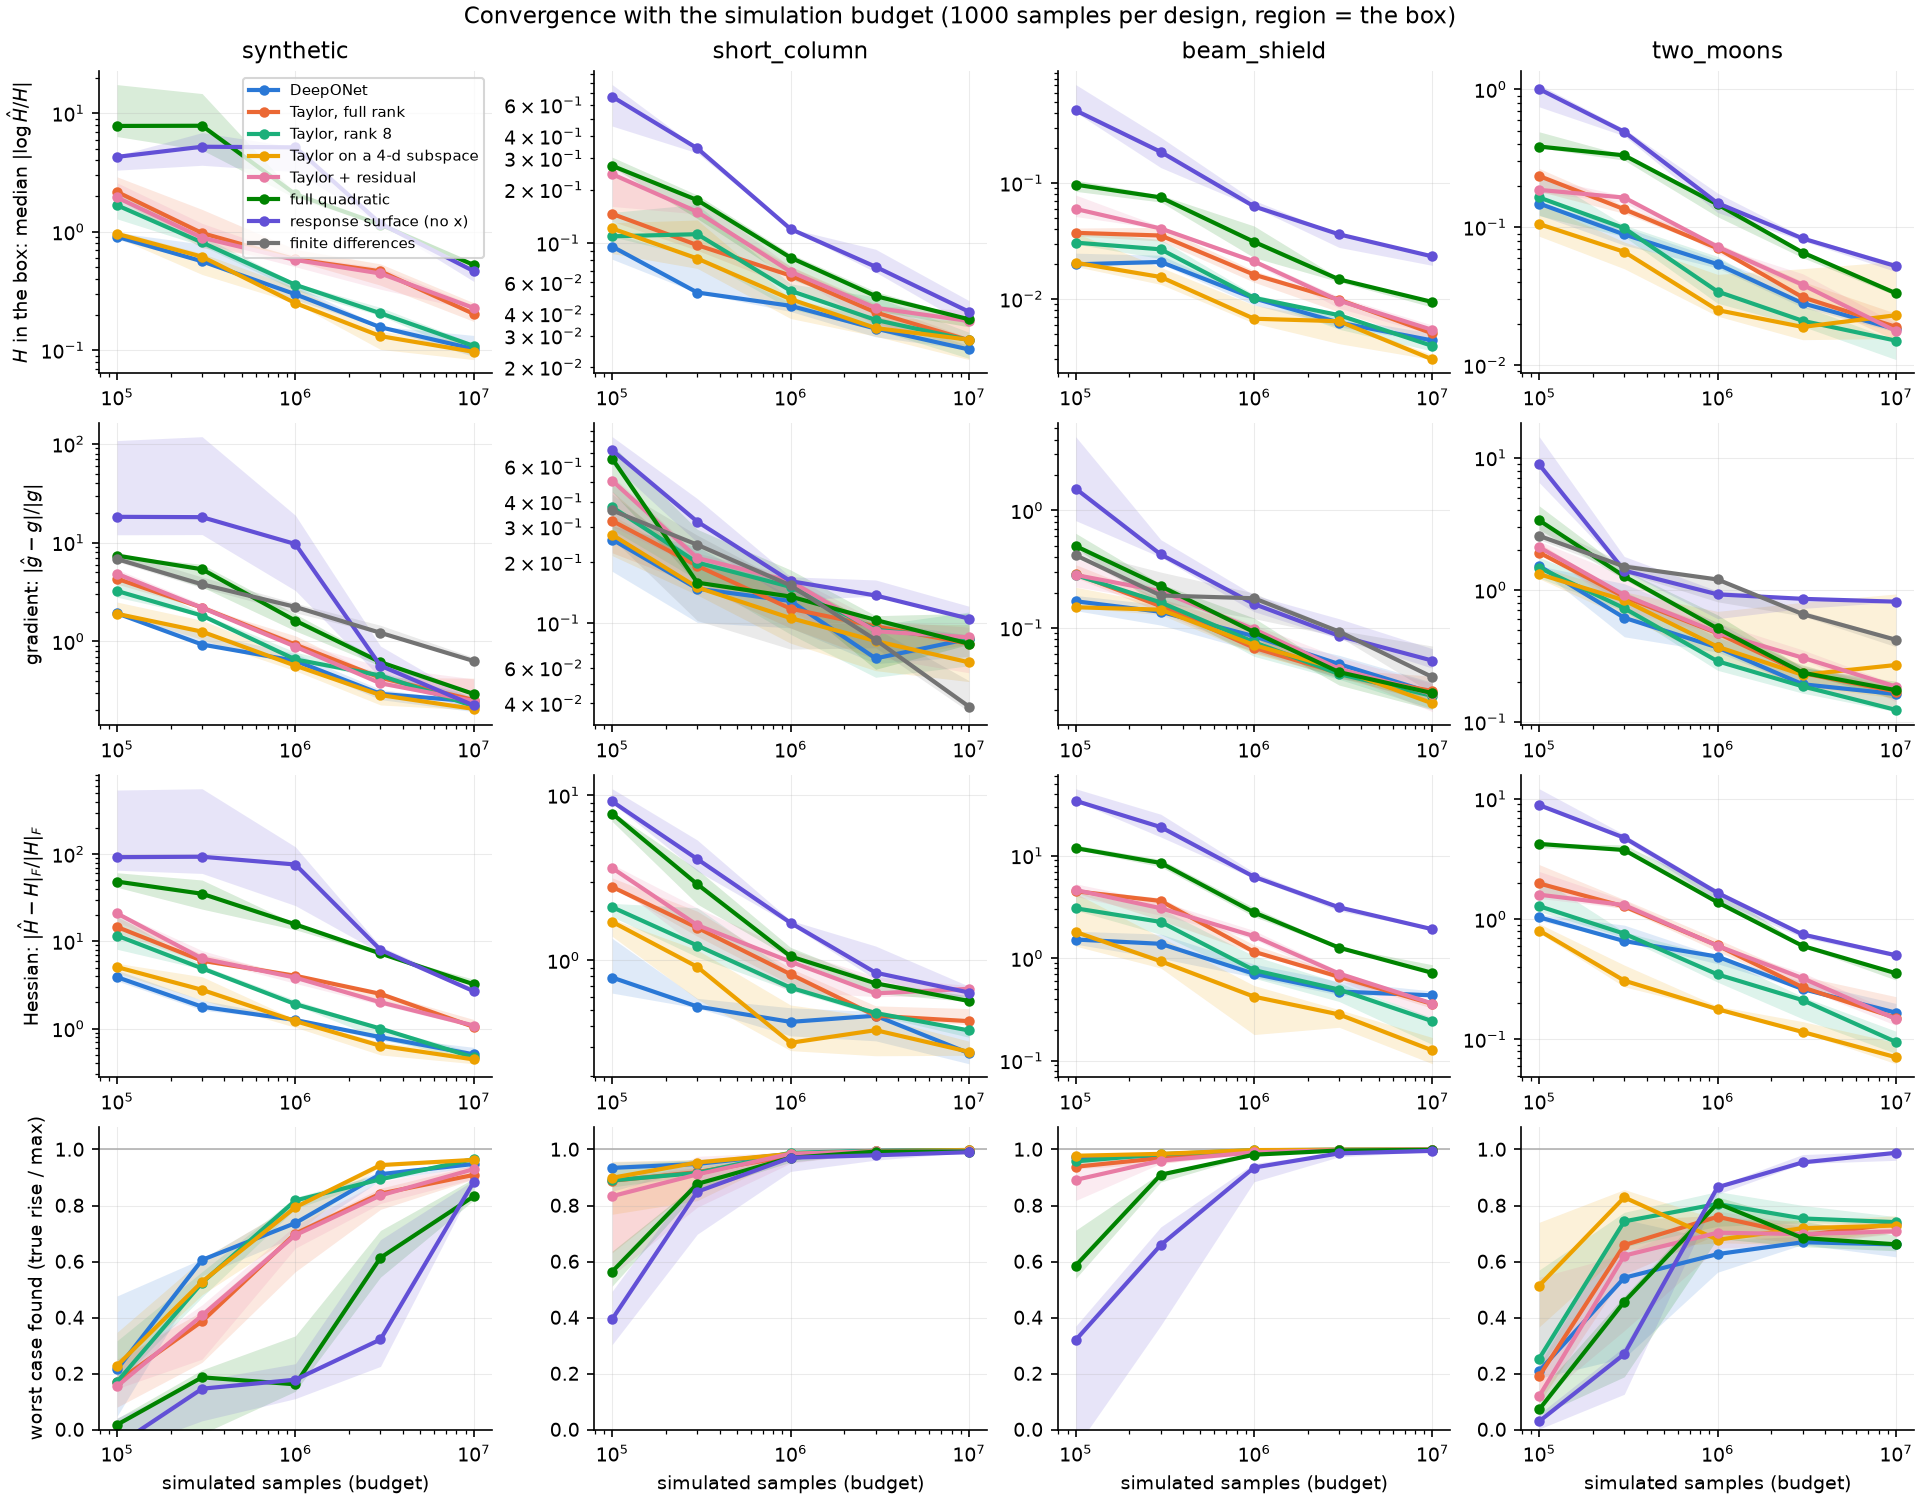
\includegraphics[width=0.53\linewidth]{round1_toy_budget.png}\hfill
  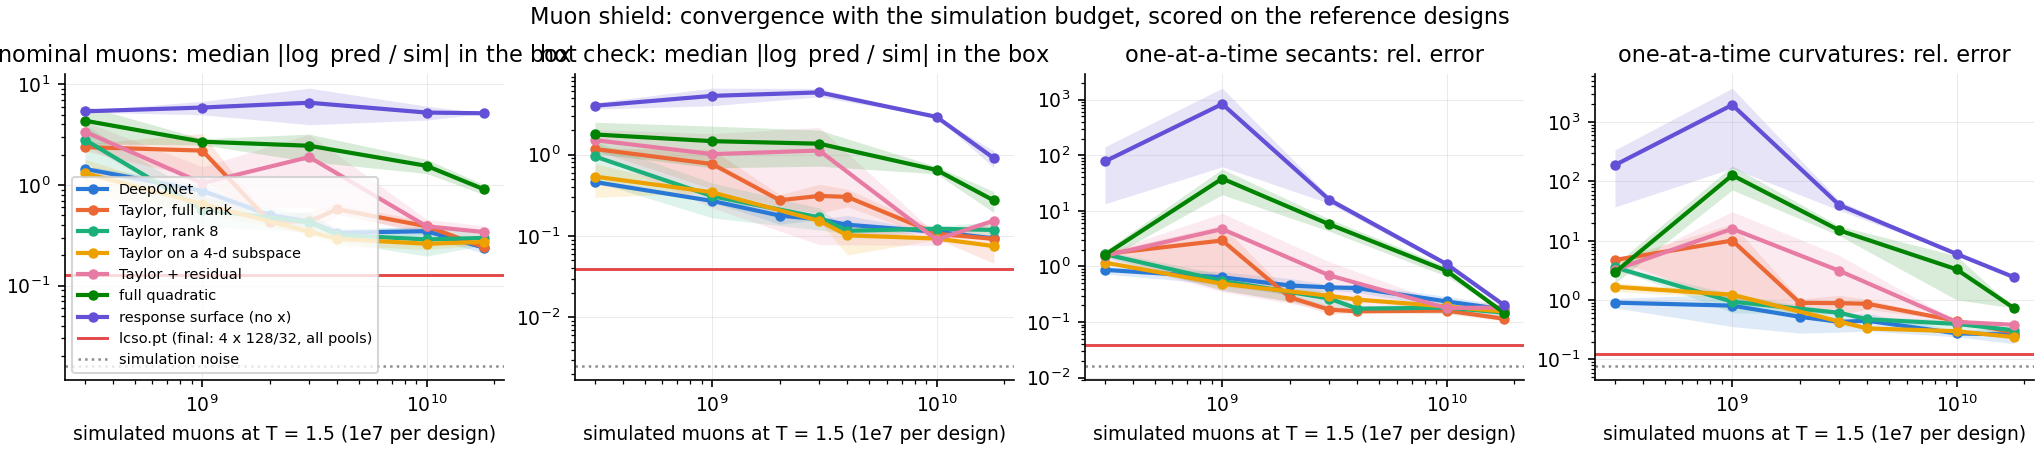
\includegraphics[width=0.45\linewidth]{round1_shield_budget.png}
  \caption{From the first analysis. Left: toy problems, errors of the hit rate, gradient and
  Hessian, and the share of the true worst case found, against the simulation budget, per
  architecture. Right: shield, errors on the reference designs against the budget (single
  models); solid red: the final surrogate of the first analysis, dotted: simulation noise.}
  \label{fig:study}
\end{figure}

\end{document}
